\documentclass[12pt]{article}
\usepackage[margin=1in]{geometry}

% TODO: Create the following new visualizations to enhance research presentation:
% 1. Multi-factor Analysis Chart: Showing interaction between model type, fusion method, and dataset
% 2. Ablation Study Visualization: Demonstrating impact of removing different components
% 3. Error Analysis Heat Map: Showing which emotion pairs are most frequently confused
% 4. Performance vs Complexity Graph: Plotting accuracy against model size/inference time
% 5. Learning Curve Comparison: Showing how different models learn over training epochs
% 6. Feature-Fusion Performance Matrix: A heatmap showing how different audio feature and fusion 
%    strategy combinations perform

% The preceding line only needs to identify funding in the first footnote. If that is unnecessary, please comment on it.
\usepackage{float}
\usepackage[table]{xcolor}
\usepackage{cite}
\usepackage{subcaption}
\usepackage{multirow}
\usepackage{graphicx}
\usepackage{amsmath,amssymb,amsfonts}
\usepackage{algorithmic}
\usepackage{graphicx}
\usepackage{textcomp}
\usepackage{xcolor}
\usepackage{multirow}
\usepackage{setspace}
\usepackage{tabularx}
\usepackage{url}
\usepackage{tabularray}
\usepackage{makecell}
\usepackage{placeins}
\usepackage{comment}
\usepackage{verbatim}
\usepackage{rotating}
\usepackage{changepage}
\renewcommand{\cellalign}{cl}

\usepackage{booktabs, multirow} % for borders and merged ranges
\usepackage{soul}% for underlines
\usepackage[table]{xcolor} % for cell colors
\usepackage{threeparttable} % for wide tables

\usepackage{pdflscape}  % For landscape environment
\usepackage{adjustbox}  % For adjustbox environment

\def\BibTeX{{\rm B\kern-.05em{\sc i\kern-.025em b}\kern-.08em
    T\kern-.1667em\lower.7ex\hbox{E}\kern-.125emX}}
    
    
    \newcommand*{\affaddr}[1]{#1} % No op here. Customize it for different styles.
\newcommand*{\affmark}[1][*]{\textsuperscript{#1}}
\newcommand*{\email}[1]{\textit{#1}}
    
\begin{document}
\begin{center}
\Large
\thispagestyle{empty}

\textbf{Two-Stage Emotion Detection from Multimodal Data}\\
\vspace{0.1in}
\large
\text{A Project Report}\\
\vspace{2in}

\text{Presented to}\\
\text{The Faculty of the Department of Computer Science}\\
\text{San Jose State University}\\

\vspace{1in}

\text{In Partial Fulfillment}\\
\text{of the Requirements for the Degree of}\\
\text{Master of Science}\\

\vspace{1in}

\text{By}\\
\text{Xiangyi Li}\\
\text{Spring 2024}\\

\end{center}

\title{}
\newpage
\thispagestyle{empty}
\begin{center}
\Large
\text{The Designated Project Committee Approves the Project Titled}\\
\vspace{0.1in}
\Large
\text{Two-Stage Emotion Detection from Multimodal Data}\\
\vspace{0.5in}
\text{by}\\
\vspace{0.1in}
\text{Xiangyi Li}\\
\vspace{1.5in}
\Large
\text{APPROVED FOR THE DEPARTMENT OF COMPUTER SCIENCE} \\
\vspace{0.1in}
\text{SAN JOSÉ STATE UNIVERSITY} \\
\vspace{0.1in}
\text{Spring 2024}\\
\vspace{1.5in}
\Large
\begin{tabular}{lcl}
Prof. Faranak Abri & \hspace{1cm} & Department of Computer Science \\
Prof. Fabio Di Troia & \hspace{1cm} & Department of Computer Science \\
Ms. Shuyi Wang & \hspace{1cm} & International Monetary Fund
\end{tabular}
 

\end{center}
\newpage

\pagenumbering{roman}
%\linespread{1.5} 

\doublespacing
\section*{Abstract}
\bigskip
Emotion detection plays a crucial role in human-computer interaction, enabling machines to recognize and respond appropriately to human emotional states. This project explores a two-stage approach to emotion detection using multimodal data, first predicting dimensional values (Arousal, Valence, Dominance) from textual and audio inputs, then mapping these representations to discrete emotion categories. We compare this approach with direct categorical classification using transformer-based language models like BERT, RoBERTa, and DeBERTa for text processing, alongside various audio feature extraction methods including MFCCs and spectrograms. 

Using the IEMOCAP dataset, we evaluate both approaches across text-only, audio-only, and multimodal configurations. Our findings reveal that while the two-stage approach provides richer emotional representations, direct classification achieves superior accuracy (91.82% with RoBERTa) compared to the two-stage method (90.13% with the same model). Interestingly, text-only approaches slightly outperform multimodal ones, though the gap narrows with optimal fusion strategies. For dimensional prediction, we observe that textual features better capture valence (positive/negative sentiment), while audio features more effectively represent arousal (emotional intensity).

This research contributes valuable insights into the tradeoffs between dimensional and categorical approaches to emotion recognition, with implications for applications requiring either maximum classification accuracy or nuanced emotional understanding. The findings suggest that application requirements should dictate the choice between these approaches, with direct classification preferred for accuracy-critical tasks and the two-stage approach for scenarios benefiting from continuous emotional representation.\\

\noindent \textbf{Keywords:} Emotion Detection, Dimensional Emotion Modeling, Natural Language Processing, Multimodal Analysis, Transformer Models
\newpage
%-------------------------------------------------------------------------------------------------
\section*{Acknowledgements}
I would like to express my sincere gratitude to my advisor, Professor Faranak Abri, for her invaluable guidance and support throughout this project. Her insights and feedback have helped me navigate challenges and achieve my goals. Thank you for your mentorship and encouragement.\\
  
\noindent
I would like to extend my gratitude to all members of my defense committee, Professor Fabio Di Troia, and Ms. Shuyi Wang.\\

\noindent  
I would like to extend my heartfelt thanks to my family and friends for their unwavering support and encouragement throughout my academic journey and in all aspects of my life.

\bigskip

\newpage
\tableofcontents
\newpage
\bigskip
\listoffigures
\listoftables


\newpage
\vspace{-0.1in}
\pagenumbering{arabic}
\section{Introduction}
\label{sec:intro}
Emotion recognition plays a fundamental role in human communication, allowing us to understand others' feelings, intentions, and needs. As artificial intelligence systems become increasingly integrated into our daily lives, the ability for machines to recognize and respond appropriately to human emotions has become crucial for meaningful human-computer interaction. This capability, often referred to as affective computing, has applications ranging from healthcare and education to entertainment and customer service.

Emotions are expressed through multiple channels, including facial expressions, voice modulations, body language, and verbal content. While humans naturally process these cues simultaneously to gauge emotional states, developing computational systems that can effectively interpret and integrate these diverse signals remains challenging. Traditional approaches often focus on a single modality, such as analyzing facial expressions or processing textual content, which limits their robustness across different contexts.

The challenge in emotion detection stems from several factors. First, emotions are inherently subjective and exist on a spectrum rather than as discrete categories. Second, emotional expressions vary considerably across individuals, cultures, and contexts. Third, different modalities may convey conflicting emotional information, requiring sophisticated fusion techniques to resolve inconsistencies. Furthermore, environmental factors like background noise or lighting conditions can significantly impact the quality of input signals.

To address these challenges, this project explores a two-stage approach to emotion detection using multimodal data. The first stage involves extracting continuous dimensional values of Arousal, Valence, and Dominance (AVD) from individual modalities—specifically text and audio features—through specialized models tailored to each data type. The second stage maps these dimensional representations to discrete emotional categories using learned boundaries and relationships between the AVD space and categorical emotions. Our hypothesis is that this two-stage approach will yield improved performance compared to direct categorical classification by leveraging the structured nature of the dimensional emotion space.

Our research makes several key contributions:
Our research makes several key contributions:

    
\section{Related Work}
\label{sec:related_work}
    
\subsection{Dimensional vs. Categorical Emotion Models}
% % Emotion recognition research has been guided by two primary theoretical frameworks: discrete categorical models and dimensional models. Categorical approaches, following Ekman's Basic Emotion Theory, classify emotions into distinct categories such as anger, happiness, and sadness. In contrast, dimensional models represent emotions as points in a continuous multi-dimensional space, with the most common dimensions being Valence (positive/negative), Arousal (active/passive), and Dominance (strong/weak).
% %     
% % Russell's Circumplex Model and the PAD (Pleasure-Arousal-Dominance) model by Mehrabian have provided theoretical foundations for dimensional approaches. These models offer advantages in representing subtle emotional variations and blended states that may not fit neatly into discrete categories. However, mapping from dimensional values to categorical labels presents challenges, as the boundaries between emotions in the dimensional space are often fuzzy and context-dependent.

% % Early computational approaches largely focused on categorical emotion recognition, but interest in dimensional modeling has grown as researchers seek to capture more nuanced emotional states. Grimm et al. pioneered continuous emotion prediction from speech, using support vector regression to estimate values along multiple emotional dimensions. More recently, Toisoul et al. demonstrated that predicting dimensional values before mapping to categories can yield improvements for facial emotion recognition. Our work extends this two-stage approach to the multimodal domain, investigating whether similar benefits can be observed when combining textual and audio inputs.

\subsection{Early Emotion-Recognition Approaches (pre-2012)}
The first wave of emotion-recognition research was dominated by lexicon and rule-based techniques such as WordNet-Affect and the NRC Emotion Lexicon. These approaches relied on predefined emotional associations of words and phrases, often lacking contextual understanding. For audio analysis, researchers extracted acoustic features like pitch, energy, and spectral characteristics, which were then processed using statistical models.

Classical machine-learning models—including Naïve Bayes, logistic regression and SVMs—were trained on bag-of-words, TF–IDF or LIWC counts for text emotion recognition, and on low-level acoustic descriptors for speech. These systems rarely exceeded approximately 60% accuracy on early benchmarks and struggled with contextual nuances and speaker variations. The limitations of these approaches stemmed largely from their inability to capture sequential patterns and higher-level semantic information.

\subsection{Deep-Learning Era (2013–2017)}
Convolutional and recurrent networks rapidly eclipsed classical models.
CNNs and \mbox{(Bi-)LSTMs} learned richer semantic and temporal features
for text, audio and vision.  In speech ER, CNN-style spectrogram
encoders combined with LSTM temporal heads pushed performance above
90 \% on Emo-DB and IEMOCAP \cite{mao2014learning}.  Hybrid CNN-LSTM
architectures similarly boosted textual ER
\cite{abdul2017emonet}.  Multimodal early-fusion CNNs that concatenate
openSMILE prosody, word embeddings and 3-D CNN facial features achieved
$\approx$80 \% on CMU-MOSI \cite{poria2018multimodal}.  Although
effective, these networks struggled with asynchronous modalities and
long-range context.

\subsection{Transformer-Based Models (2018–2025)}
Contextualised language models revolutionised unimodal ER.  Fine-tuning
BERT, RoBERTa or DeBERTa yields state-of-the-art textual accuracies on
many datasets \cite{liu2019roberta}.  Cross-modal transformers extend
self-attention to heterogeneous streams.  \textsc{MulT}
\cite{tsai2019mult} attends across mis-aligned audio, visual and
linguistic tokens, attaining 84.8 \% unweighted accuracy (UA) on the
six-class IEMOCAP task.  Progressive-modality reinforcement
\cite{lv2021progressive} iteratively re-weights modalities, while
TransModality \cite{wang2020context} unifies feature extraction and
fusion within one transformer backbone.  Self-supervised encoders such
as Wav2Vec 2.0 supply powerful speech features that, when fused with
RoBERTa text embeddings, reach 84.7 \% UA on IEMOCAP and 64 \% F1 on the
challenging MELD corpus \cite{siriwardhana2020joint}.

\subsection{Multimodal Fusion Taxonomy}
Fusion strategies fall into three categories:

\textbf{Early fusion} concatenates raw features before a shared
classifier \cite{poria2017review}.  It captures low-level correlations
but ignores modality structure.

\textbf{Late fusion} trains modality-specific classifiers whose logits
are fused by averaging or a meta-learner
\cite{wang2019words}.  Flexibility is high, yet fine-grained
interactions are lost.

\textbf{Hybrid / fine-grained fusion} combines both.  Tensor Fusion
Networks \cite{zadeh2018multimodal_tfn}, Memory Fusion Networks
\cite{zadeh2018mfn}, capsule-based interaction
\cite{wang2019words} and cross-modal transformers
\cite{tsai2019mult} explicitly model inter-modal dynamics and achieve
the best overall results (e.g., 89 \% accuracy on CMU-MOSEI
\cite{mittal2020m3er}).

\subsection{Benchmark Datasets}
\textbf{IEMOCAP} \cite{busso2008iemocap} remains the de-facto benchmark
($\sim$10 k utterances, 9 emotions, audio+video+transcripts).  
\textbf{CMU-MOSI} \cite{zadeh2016mosi} and
\textbf{CMU-MOSEI} \cite{zadeh2018multimodal} provide large
"in-the-wild'' video reviews with sentiment and six-emotion labels.
\textbf{MELD} \cite{poria2018meld} introduces multi-party dialogue
context; \textbf{RAVDESS} \cite{livingstone2018ravdess} supplies
balanced acted speech.  Each poses distinct challenges in spontaneity,
noise and class imbalance, motivating the use of unweighted metrics
(UAR, UF1) alongside accuracy and weighted F1.

\subsection{Current Challenges}
Despite progress, open problems persist: domain shift (lab $\rightarrow$
wild) causes 15–20 pp degradation; demographic bias is under-studied;
conversation-level understanding and real-time, low-resource deployment
remain difficult.  Addressing these issues requires larger,
diversified corpora and efficient, bias-aware models.

\clearpage
\begin{table}[p]
\sffamily\tiny
\centering
\caption{Comparison of Emotion Detection Models (Multimodal, Text, Audio)}
\renewcommand{\arraystretch}{0.85}
\setlength{\tabcolsep}{1.8pt}
\begin{adjustbox}{width=\textwidth,center}
\begin{tabular}{@{}p{2.3cm}p{1.6cm}p{1.2cm}p{2.4cm}p{2.3cm}p{1.1cm}p{2.1cm}@{}}
\toprule
\textbf{Reference} & \textbf{Dataset} & \textbf{Modality} & \textbf{Features} & \textbf{Classification} & \textbf{Metric} & \textbf{Performance} \\
\midrule
Poria et al. (2017) & CMU-MOSI (binary) & S+T+V & openSMILE, word2vec, 3D-CNN & Early fusion (feature concat) & Acc & 81.3\% \\
Liu et al. (2018) & IEMOCAP (4) & S+T+V & COVAREP, GloVe, FACET & Utterance interaction (memory) & UF1 & 83.1\% \\
Zadeh et al. (2018) & YT(3), MOUD(2), IEMOCAP(9) & S+T+V & COVAREP, GloVe, FACET & Fine-grained interaction (tensor) & Acc/F1 & YT: 61.0\%/60.7\%; MOUD: 81.1\%/80.4\%; IEMO: 36.5\%/34.9\% \\
Pham et al. (2019) & CMU-MOSI (binary) & S+T+V & MFCC, GloVe, FACET+OpenFace & Fine-grained interaction & Acc/F1 & 76.5\%/73.4\% \\
Poria et al. (2018) & IEMOCAP(4), MOUD(2), MOSI(2) & S+T+V & openSMILE, CNN, 3D-CNN & Early fusion (multimodal CNN) & Acc & IEMO: 71.6\%; MOUD: 67.9\%; MOSI: 76.7\% \\
Zadeh et al. (2018) & CMU-MOSEI (6) & S+T+V & COVAREP, GloVe, MTCNN & Fine-grained (dynamic fusion) & UAcc/UF1 & 62.4\%/76.3\% \\
Majumder et al. (2018) & MOSI(2), IEMOCAP(4) & S+T+V & openSMILE, word2vec, 3D-CNN & Hierarchical fusion w/ context & Acc & MOSI: 80.0\%; IEMO: 76.5\% \\
Tsai et al. (2019) & ICT-MMMO(2), YT(3), MOUD(2), IEMOCAP(6) & S+T+V & COVAREP, GloVe, FACET & Cross-modal Transformer (MULT) & Acc/F1 & ICT: 81.3\%/79.2\%; YT: 53.3\%/52.4\%; MOUD: 82.1\%/81.7\%; IEMO: 84.8\%(UAcc)/81.4\%(UF1) \\
Wang et al. (2019) & IEMOCAP (4) & S+T+V & COVAREP, GloVe, FACET & Fine-grained (Capsule network) & UAcc/UF1 & 81.9\%/81.2\% \\
Tsai et al. (2018) & IEMOCAP (4) & S+T+V & COVAREP, GloVe, FACET & Factorized multimodal rep. & UAcc/UF1 & 74.7\%/71.5\% \\
Pham et al. (2020) & ICT-MMMO(2), YT(2) & S+T+V & COVAREP, GloVe, FACET & Fine-grained interaction & Acc/F1 & ICT: 81.3\%/80.8\%; YT: 51.7\%/52.4\% \\
Liang et al. (2021) & IEMOCAP(4), MELD(7) & S+T+V & openSMILE, BERT, DenseNet & Simple feature concat & Acc/F1 & IEMO: 75.6\%(UAcc 74.5\%); MELD: 57.1\%(F1) \\
Mittal et al. (2021) & IEMOCAP(4), MOSEI(6) & S+T+V & MFCC/pitch, GloVe, facial AUs & Fine-grained (CNN+LSTM) & Acc/F1 & IEMO: 82.7\%/82.4\%; MOSEI: 89.0\%/80.2\% \\
Wang et al. (2020) & IEMOCAP(6), MOSI(2), MELD(7) & S+T+V & openSMILE, CNN, 3D-CNN & End-to-end Transformer & Acc & IEMO: 60.8\%; MELD: 62.0\%; MOSI: 82.7\% \\
Sun et al. (2020) & IEMOCAP (4) & S+T+V & COVAREP, BERT, FACET & Deep CCA (correlation) & UAcc/UF1 & 83.0\%/81.8\% \\
Siriwardhana (2020) & IEMOCAP(4), MELD(7) & S+T+V & Wav2Vec, RoBERTa, FabNet & Transformer-based late fusion & UAcc/F1 & IEMO: 84.7\%/84.2\%; MELD: 64.3\%/63.9\% \\
Lv et al. (2021) & IEMOCAP(4), MOSI(2) & S+T+V & COVAREP, BERT, FACET & Progressive modality reinforce & UAcc/UF1 & IEMO: 85.1\%/83.8\%; MOSI: 83.6\%/83.4\% \\
Majumder et al. (2019) & MELD (7) & T(conv) & GloVe, context state & GRU-based RNN (party-state) & WF1 & 57.0\% \\
Ghosal et al. (2019) & MELD (7) & T(conv) & GloVe, speaker depend. & Graph convolution network & WF1 & 58.1\% \\
Ghosal et al. (2020) & MELD (7) & T(conv) & RoBERTa, commonsense & Transformer + commonsense & WF1 & 65.2\% \\
Trinh et al. (2022) & IEMOCAP (4) & A & Mel spectrogram, spectral feat. & CNN + GRU (ensemble) & Acc & 97.47\% \\
Issa et al. (2020) & RAVDESS (8) & A & MFCC, spectral contrast, mel-spec & Deep NN (fully-connected) & Acc & 71.6\% \\
Bautista et al. (2021) & RAVDESS (8) & A & Augmented spectrograms & Parallel CNN–Transformer & Acc & 89.33\% \\
Pan et al. (2022) & IEMOCAP (4) & A & MFCC features & CNN + LSTM hybrid & Acc & 96.21\% \\
\bottomrule
\end{tabular}
\end{adjustbox}
\vspace{1mm}
\begin{flushleft}
{\tiny Note: S=Speech, T=Text, V=Visual, A=Audio, Acc=Accuracy, UF1=Unweighted F1, WF1=Weighted F1, YT=YouTube, IEMO=IEMOCAP}
\end{flushleft}
\end{table}
\clearpage

\subsection{Audio-Based Emotion Detection}
% % Audio-based emotion recognition has traditionally focused on extracting acoustic features that correlate with emotional states. Low-level descriptors (LLDs) such as pitch, energy, formants, and voice quality parameters were among the earliest features explored~\cite{schuller2009acoustic}.

% % Mel-Frequency Cepstral Coefficients (MFCCs), originally developed for speech recognition, have proven effective for emotion detection by capturing the spectral envelope of speech~\cite{li2013speech}. Similarly, spectrograms provide time-frequency representations that preserve temporal dynamics important for emotion recognition.

% % With deep learning, Convolutional Neural Networks (CNNs) have been applied directly to spectrograms, treating them as images and learning relevant patterns automatically~\cite{mao2014learning}. This approach eliminates the need for handcrafted feature engineering while often improving performance.

% % More recently, self-supervised approaches like wav2vec~\cite{schneider2019wav2vec} have gained attention by learning representations from unlabeled audio data. These models capture nuanced acoustic properties that may be missed by traditional feature extraction methods.

\subsection{Multimodal Approaches}
Recognizing that emotions are expressed through multiple channels, researchers have increasingly focused on multimodal approaches. These methods face the challenge of effectively combining information from different modalities that may operate at different time scales and granularities.

Early fusion (feature-level) combines raw features or low-level representations before classification, allowing the model to learn joint patterns across modalities~\cite{poria2017review}. While conceptually simple, this approach must handle different feature dimensions and time scales.

Late fusion (decision-level) processes each modality independently and combines their predictions, typically through voting schemes, weighted averaging, or additional classifiers~\cite{wagner2011introducting}. This approach is more modular but may miss cross-modal interactions.

Hybrid fusion combines aspects of both early and late fusion, often using attention mechanisms to dynamically weight different modalities based on their relevance~\cite{zadeh2018memory}. These approaches have shown promising results by adapting to varying reliability of modalities across different inputs.

Transformer-based models have recently been extended to the multimodal domain, with architectures like MMBT~\cite{kiela2019supervised} jointly encoding textual and visual information. These approaches leverage the self-attention mechanism to capture relationships both within and across modalities.

\subsection{Emotion Recognition Datasets}
Several benchmark datasets have been developed for emotion recognition research. The Interactive Emotional Dyadic Motion Capture (IEMOCAP) dataset~\cite{busso2008iemocap} contains audio-visual recordings of acted dialogues, annotated for categorical emotions and dimensional affect labels. It has become one of the most widely used resources for multimodal emotion recognition.

Other notable datasets include SEMAINE~\cite{mckeown2012semaine}, which features interactions between humans and artificially intelligent agents; RAVDESS~\cite{livingstone2018ryerson}, containing emotional speech and song; and CMU-MOSEI~\cite{zadeh2018multimodal}, which includes YouTube video clips with sentiment and emotion annotations.

Our work builds upon these foundations by systematically comparing state-of-the-art transformer models for text processing, exploring various audio feature representations, and evaluating different fusion strategies on the IEMOCAP dataset.

\section{Methodology}
\label{sec:methodology}
Our approach to emotion detection employs a two-stage architecture that first predicts dimensional emotion values (Arousal, Valence, Dominance) from textual and audio modalities separately, then maps these dimensional representations to discrete emotion categories. This section provides a comprehensive overview of our methodology, including detailed descriptions of model architectures, audio feature extraction techniques, training procedures, and the mapping process between dimensional and categorical representations.

\subsection{System Architecture Overview}
Figure~\ref{fig:system_architecture} illustrates the high-level architecture of our two-stage emotion detection system. The first stage consists of separate processing pipelines for textual and audio data, each optimized for the specific characteristics of its modality and trained to predict continuous AVD values. The second stage implements a mapping function that translates the predicted dimensional values into discrete emotion categories, leveraging the structured nature of the dimensional emotion space.

\begin{figure}[h]
    \centering
    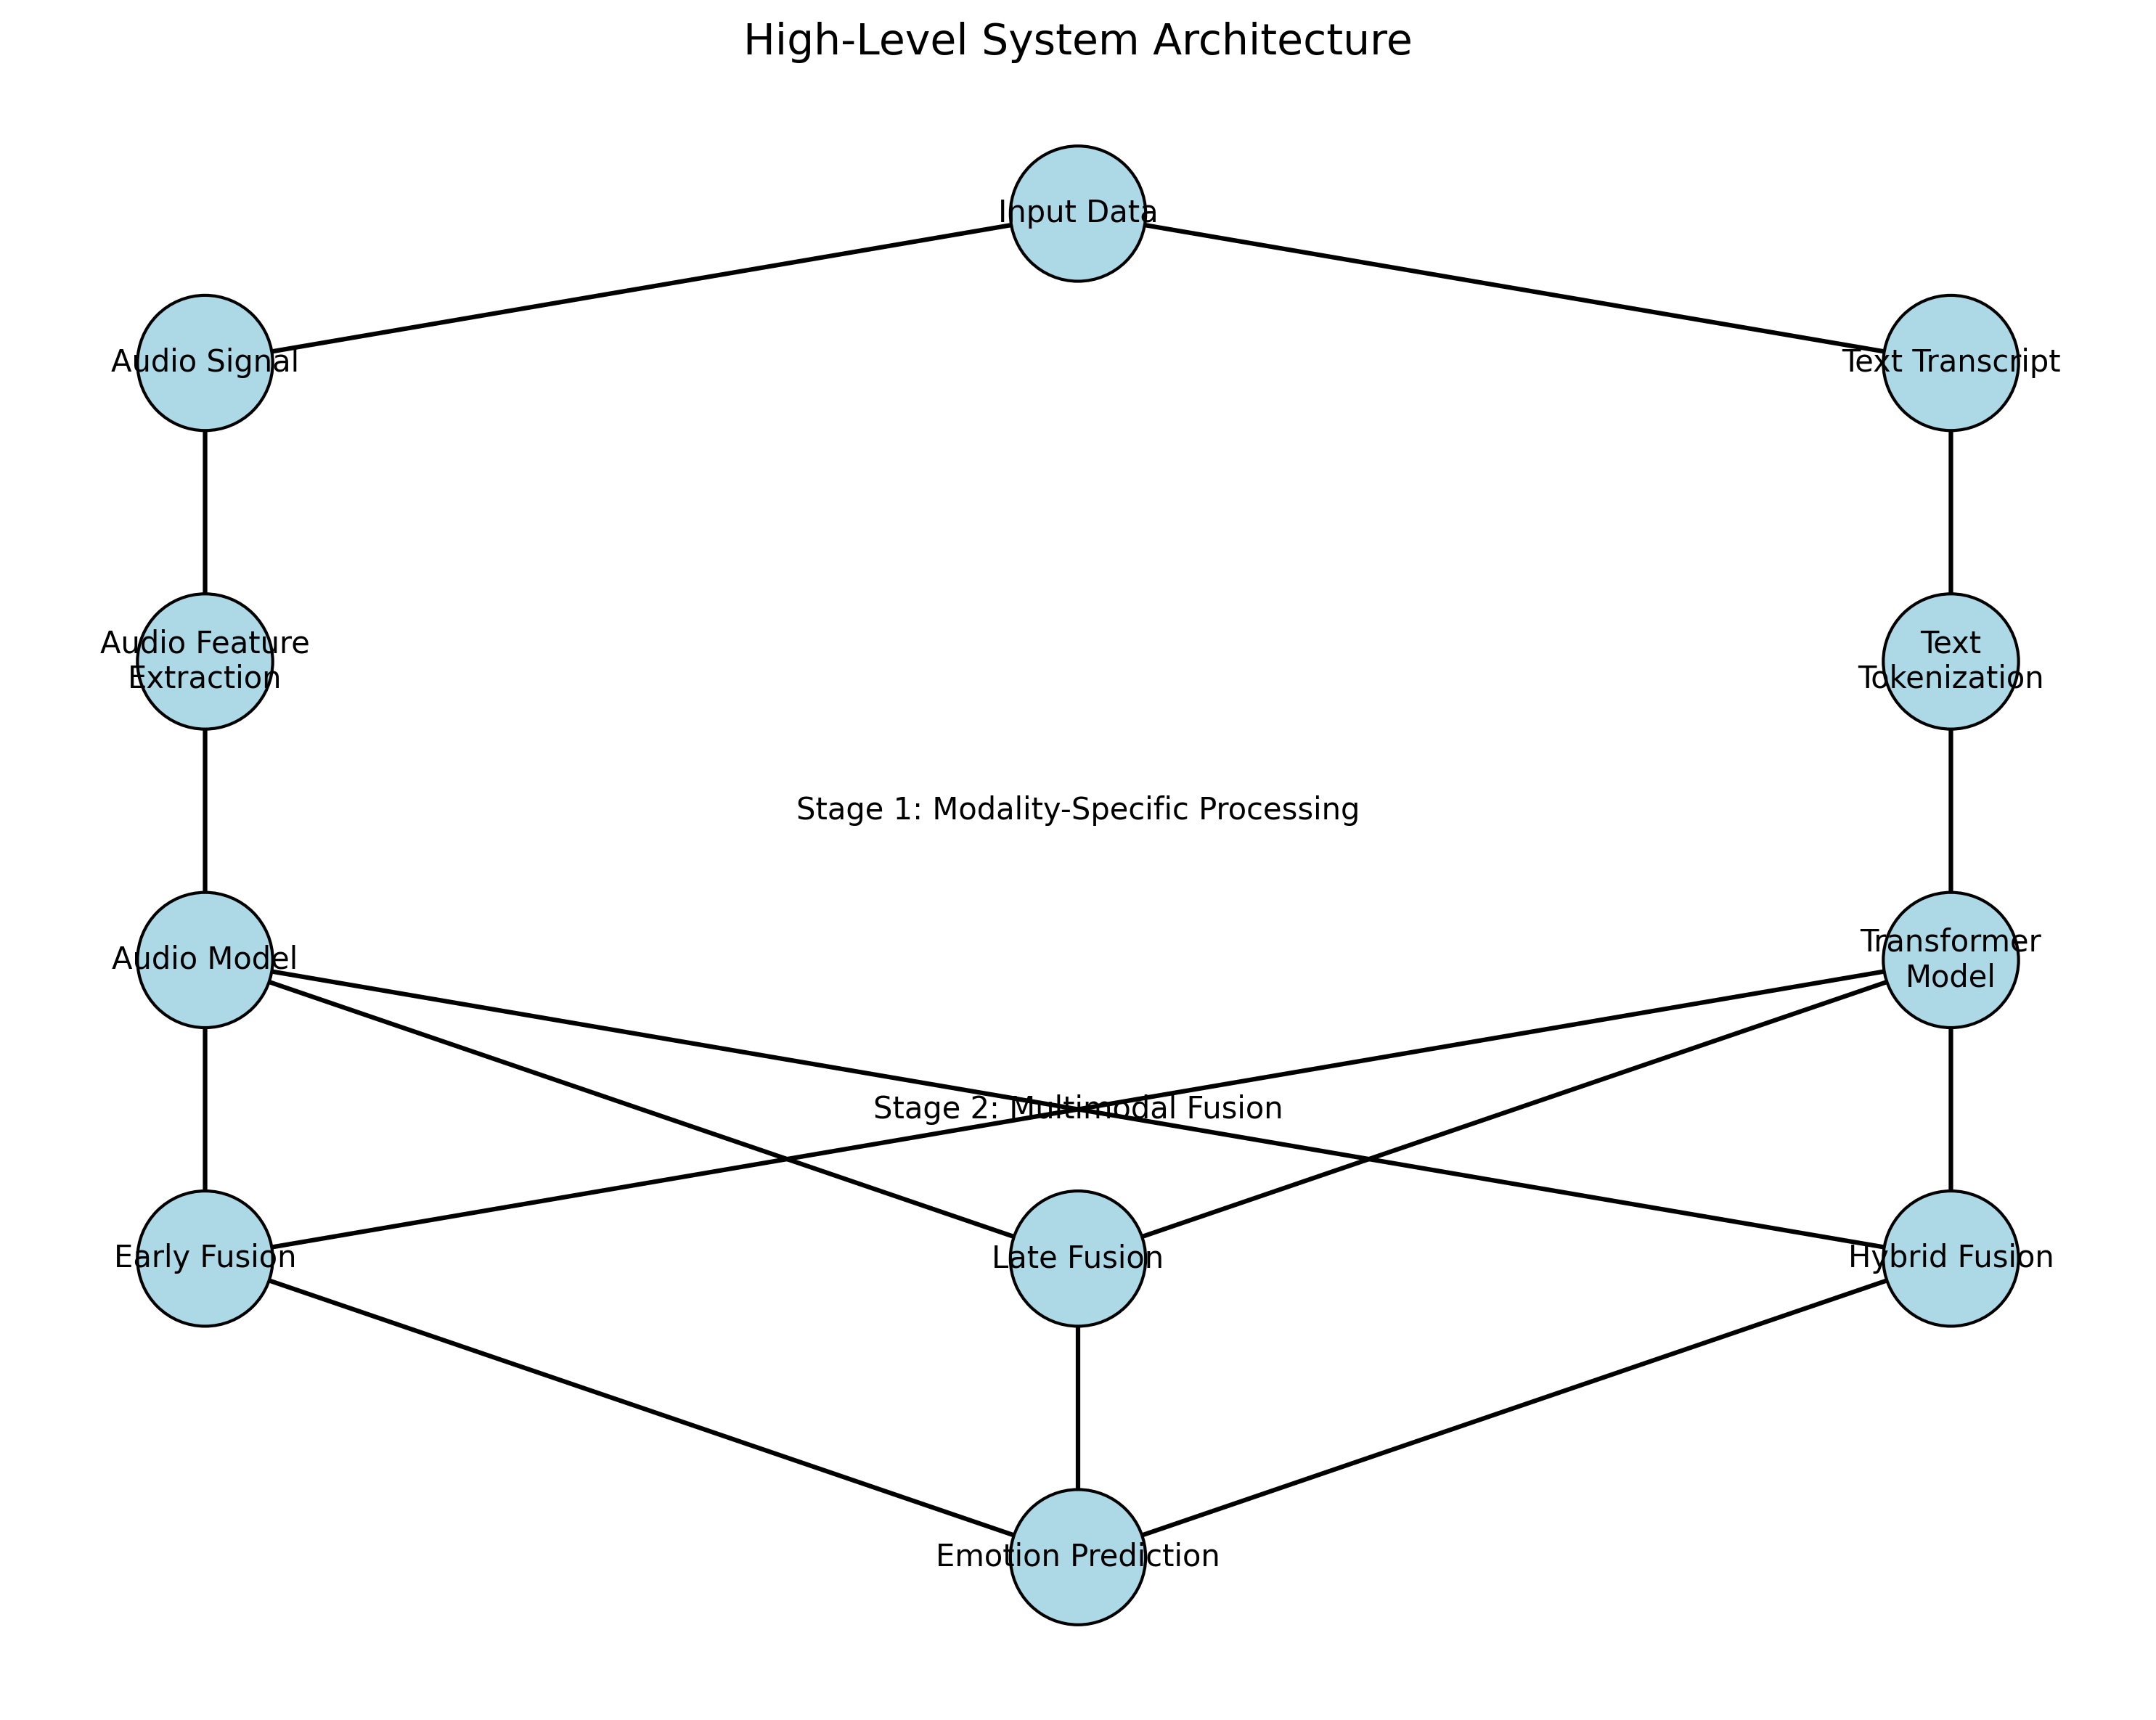
\includegraphics[width=0.9\linewidth]{Figures_Improved/system_architecture_fixed.png}
    \caption{System architecture of the two-stage emotion detection model.}
    \label{fig:system_architecture}
\end{figure}

This two-stage design offers several advantages over direct categorical classification. First, it acknowledges the continuous nature of emotional states by modeling them initially in a dimensional space. Second, it allows for more nuanced representations of emotional states that may not perfectly align with discrete categories. Third, it enables better interpretability by providing dimensional values that have psychological meaning beyond category labels. Finally, the intermediate dimensional representation can potentially capture subtle emotional variations that categorical approaches might miss.

The design is also modular, offering flexibility to handle independent optimization of each modality's processing pipeline, experimentation with different combinations of models, and the ability to handle missing modalities by falling back to single-modality predictions. This approach enhances interpretability through analysis of each modality's contribution to the dimensional predictions and the subsequent mapping to categories.

\subsection{Text Processing Models}
For processing textual data, we evaluated several state-of-the-art transformer-based models. Each model was implemented using the Hugging Face Transformers library, with a classification head added on top of the base model for predicting dimensional emotion values (AVD).

\subsubsection{BERT (Bidirectional Encoder Representations from Transformers)}
BERT~\cite{devlin2018bert} revolutionized NLP by introducing bidirectional context modeling through a masked language modeling objective. The model architecture consists of multiple transformer encoder layers that process tokens in parallel, with each token attending to all other tokens in the sequence. Specifically, the \texttt{bert-base-uncased} variant we used has 12 transformer encoder layers, a hidden size of 768 dimensions, and 12 attention heads, totaling approximately 110 million parameters. It supports a maximum sequence length of 512 tokens and uses a vocabulary of 30,522 tokens. BERT's pre-training relied on two objectives: Masked Language Modeling (MLM), where 15% of input tokens are randomly masked and predicted based on bidirectional context, and Next Sentence Prediction (NSP), predicting whether two sentences appear consecutively in the original text.

For AVD prediction, we extracted the final hidden state of the [CLS] token, which serves as an aggregate representation of the entire input sequence. This representation was passed through a regression head appropriate for predicting the three continuous AVD values.

\subsubsection{RoBERTa (Robustly Optimized BERT Approach)}
RoBERTa~\cite{liu2019roberta} builds upon BERT with several optimizations to the training methodology while maintaining the same core architecture. Key improvements include eliminating the NSP objective, using dynamic masking patterns where new masks are generated each time a sequence is presented, training on longer sequences, employing significantly larger batch sizes (8K sequences), and utilizing a much larger pre-training corpus (160GB vs. BERT's 16GB). The \texttt{roberta-base} variant we used has the same architecture as BERT-base (12 layers, 768 hidden size, 12 attention heads) but uses a larger vocabulary of 50,265 tokens based on byte-level Byte Pair Encoding (BPE) and comprises 125 million parameters. We used the \texttt{RobertaForSequenceClassification} class, adapting its head for AVD regression and fine-tuned all layers during training.

\subsubsection{XLNet}
XLNet~\cite{yang2019xlnet} introduces a generalized autoregressive pre-training method called Permutation Language Modeling. This approach captures bidirectional context by predicting tokens in a random order, avoiding BERT's potentially limiting assumption of independence between masked tokens. It also employs a two-stream self-attention mechanism (query stream and content stream) to prevent target information leakage during training. The \texttt{xlnet-base-cased} variant consists of 12 transformer layers, a hidden size of 768, 12 attention heads, and 110 million parameters. We utilized the \texttt{XLNetForSequenceClassification} model, adapted for AVD regression, maintaining consistent hyperparameters for fair comparison.

\subsubsection{ALBERT (A Lite BERT)}
ALBERT~\cite{lan2019albert} addresses BERT's parameter inefficiency through significant parameter-reduction techniques while aiming to maintain performance. It employs factorized embedding parameterization, decomposing the large vocabulary embedding matrix into two smaller matrices, and cross-layer parameter sharing, using the same parameters across all transformer layers. The \texttt{albert-base-v2} variant, despite having 12 transformer layers and a hidden size of 768, contains only about 12 million parameters (roughly 10% of BERT-base). ALBERT also replaces NSP with Sentence Order Prediction (SOP), a more challenging task focused on inter-sentence coherence, and uses a dropout rate of 0 on the embedding layer.

\subsubsection{ELECTRA (Efficiently Learning an Encoder that Classifies Token Replacements Accurately)}
ELECTRA~\cite{clark2020electra} introduces a more sample-efficient pre-training approach using a generator-discriminator architecture. A small generator model (similar to BERT) produces plausible replacements for masked input tokens. The main ELECTRA model, the discriminator, is then trained on a replaced token detection (RTD) task: classifying each token in the sequence as either "original" or "replaced" by the generator. This approach is more efficient because the loss is computed over all input tokens, not just the masked ones, leading to faster convergence and stronger representations. We used the \texttt{google/electra-base-discriminator} variant (12 layers, 768 hidden size, 110 million parameters), adapting its output for AVD regression.

\subsubsection{DeBERTa (Decoding-enhanced BERT with disentangled attention)}
DeBERTa~\cite{he2020deberta} enhances BERT with two key innovations: disentangled attention and an enhanced mask decoder. Disentangled attention computes attention weights using separate vectors for word content and relative position, providing a more nuanced way to model token relationships. The enhanced mask decoder incorporates absolute positional information in the final decoding layer to further refine predictions. We used the \texttt{microsoft/deberta-v3-base} variant, which includes further improvements like a new vocabulary based on SentencePiece. This model has 12 layers, a hidden size of 768, and 184 million parameters. We adapted the \texttt{DebertaV2ForSequenceClassification} model for our AVD prediction task.

\subsection{Text Model Training Procedure}
All transformer models followed a consistent training procedure to ensure fair comparison:

\paragraph{Preprocessing:}
\begin{enumerate}
    \item Tokenization using model-specific tokenizers
    \item Truncation/padding to a maximum sequence length of 128 tokens
    \item Creation of attention masks to differentiate between actual tokens and padding
\end{enumerate}

\paragraph{Hyperparameters:}
    Learning rate: 2e-5 with linear decay
    Batch size: 16 samples
    Training epochs: 40 (with early stopping based on validation loss)
    Optimizer: AdamW with weight decay of 0.01
    Gradient clipping: Maximum gradient norm of 1.0
    Warmup: 10\% of total training steps

\paragraph{Regularization Techniques:}
    Early stopping: Training halted when validation loss failed to improve for 5 consecutive epochs
    Dropout: Default dropout rate of 0.1 in transformer layers
    Weight decay: Applied to all parameters except biases and layer normalization

\paragraph{Loss Function:}
For discrete emotion categories, we used cross-entropy loss. For dimensional emotion recognition (valence, arousal, dominance), we employed mean squared error (MSE) loss.

\subsection{Audio Feature Extraction}
The audio modality provides crucial information about emotional states through prosodic patterns, voice quality, and spectral characteristics. We explored four different audio representation techniques, each capturing different aspects of the speech signal and used as input for AVD prediction models.

\subsubsection{Mel-Frequency Cepstral Coefficients (MFCCs)}
MFCCs are perceptually motivated spectral features that represent the short-term power spectrum of sound, mimicking the human auditory system's frequency response. The extraction process begins with pre-emphasis using a high-pass filter to boost high frequencies. The audio is segmented into short frames (25ms with 10ms stride), and a Hamming window is applied to each frame to reduce spectral leakage. The Fast Fourier Transform (FFT) is computed to obtain the power spectrum, followed by applying a mel-scale filter bank (40 filters) to mimic human hearing. The logarithm of filter bank energies is taken, and the Discrete Cosine Transform (DCT) is applied to decorrelate features. We retained the first 40 coefficients. This process was implemented using the Librosa library (version 0.9.1) with audio resampled to 16kHz. The final MFCC features were Z-score normalized.

\begin{figure}[h]
    \centering
    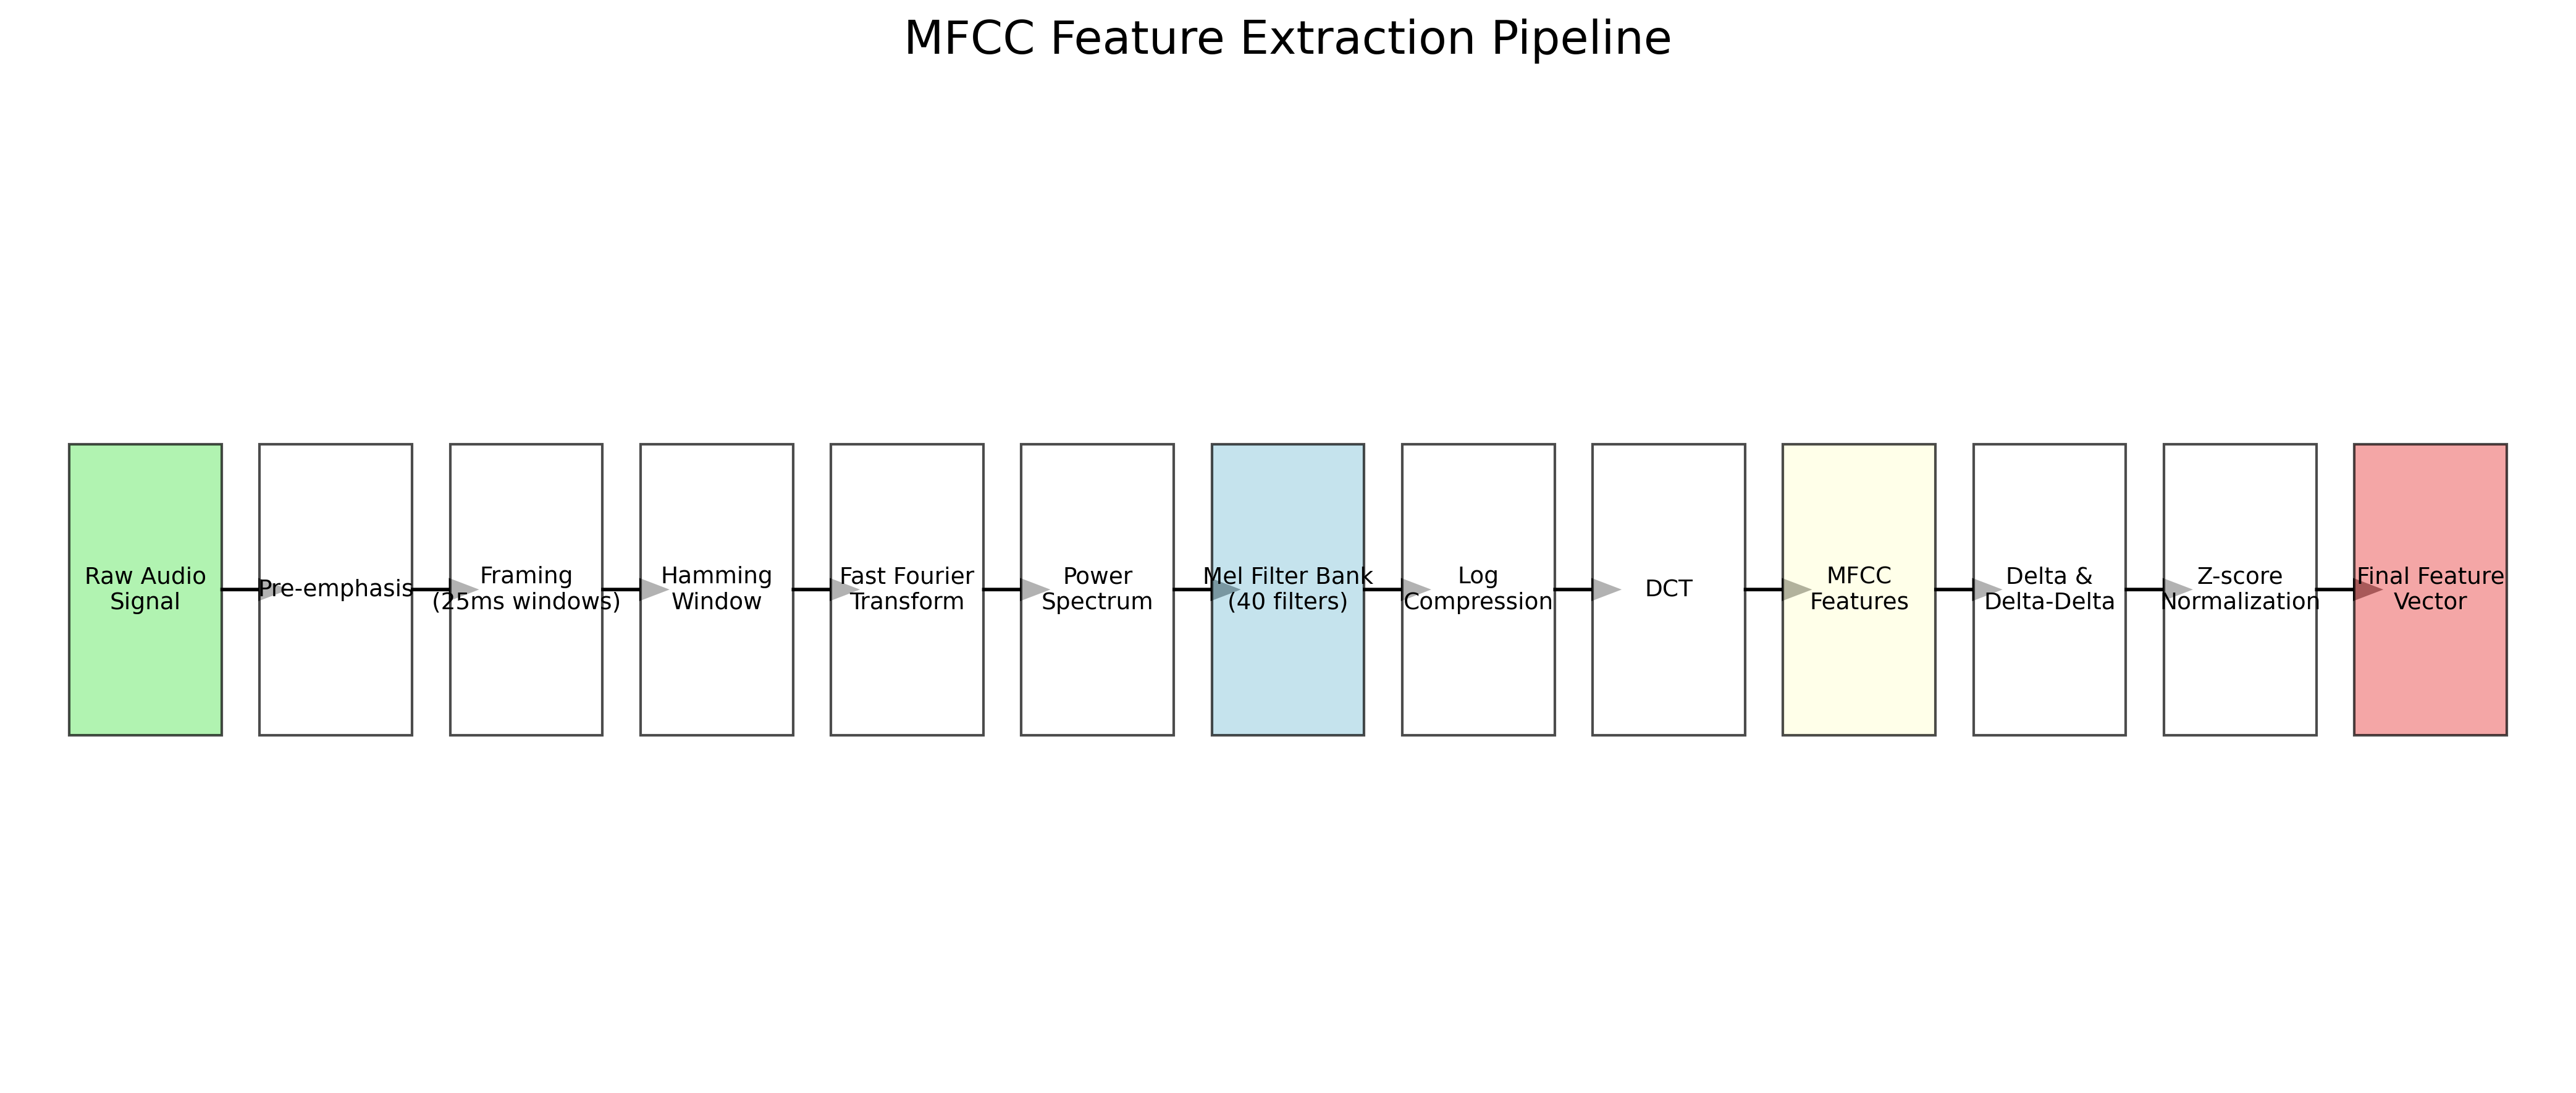
\includegraphics[width=1.0\linewidth]{Figures_Improved/mfcc_pipeline.png}
    \caption{System architecture of the two-stage emotion detection model.}
    \label{fig:mfcc_pipeline}
\end{figure}

\subsubsection{Spectrograms}
Spectrograms provide a visual representation of frequencies in an audio signal over time, preserving both frequency and temporal dynamics important for emotion recognition. Their generation involves segmenting the audio into overlapping frames (25ms with 10ms stride) and applying a Hamming window. The Short-Time Fourier Transform (STFT) is computed, and its magnitude is calculated. This magnitude spectrum is then converted to the mel scale using 128 mel bins covering the 0-8kHz frequency range. Finally, logarithmic compression is applied. We used Librosa for extraction and normalized the resulting spectrograms (Time frames × 128 mel bins) using min-max scaling to [0,1] before feeding them as single-channel grayscale images to CNN models.

\subsubsection{Prosodic Features}
Prosodic features capture rhythm, stress, and intonation aspects of speech that often correlate strongly with emotional states. Our feature set included statistics (mean, std, min, max, range) of the fundamental frequency (F0 or pitch contour) and frame-level energy. We also incorporated measures like speaking rate, voice quality metrics (jitter, shimmer, harmonics-to-noise ratio), and rhythm metrics (pauses, articulation rate). These features were extracted using Librosa and Parselmouth, computed over 25ms frames with a 10ms shift, and statistical functionals were applied over 500ms windows with 250ms overlap. The resulting 88 features per utterance were Z-score normalized based on training set statistics. Due to implementation challenges described later, these features were not used in our final best models.

\subsubsection{Wav2vec Embeddings}
Wav2vec~\cite{schneider2019wav2vec} represents a self-supervised approach for learning representations directly from raw audio waveforms. Its architecture consists of an encoder network using temporal convolutions to convert raw audio into latent representations, and a context network capturing sequential context through additional convolutional layers. It is pre-trained using a contrastive prediction task. We utilized the \texttt{wav2vec-large} model pre-trained on LibriSpeech to extract 512-dimensional embeddings, generating one vector per 10ms of audio. These embeddings were aggregated using attention pooling and processed through bidirectional LSTM layers. Similar to prosodic features, integration issues prevented the successful inclusion of Wav2vec features in our top-performing configurations.

\subsection{Audio Processing Models}
Different audio features require specialized model architectures for effective processing to predict AVD values. We implemented two main types of models: convolutional networks for 2D representations like spectrograms and reshaped MFCCs, and recurrent networks for sequential features such as prosodic features and wav2vec embeddings, although the latter two feature types were ultimately not part of our best-performing models due to implementation challenges.

\subsubsection{CNN for Spectrograms and MFCCs}
For 2D representations (spectrograms or MFCCs reshaped into a 2D format), we employed a convolutional neural network (CNN) inspired by successful architectures in audio classification tasks. The input, either a spectrogram or reshaped MFCC features (Time frames × Frequency bins), was processed through four convolutional blocks. Each block consisted of a 2D convolution with 3×3 kernels, followed by batch normalization, ReLU activation, and max-pooling (2×2). The number of filters progressed through 32, 64, 128, and 256 across these blocks. The output from the convolutional blocks was then flattened and passed through two fully connected layers: one with 512 units and ReLU activation, and a second with 128 units and ReLU activation. Finally, an output layer predicted the AVD values. This CNN was implemented in PyTorch, with dropout (0.5) applied after the first fully connected layer for regularization and He initialization for convolutional layers. We used a batch size of 32 and the Adam optimizer with a learning rate of 0.0001.

\subsubsection{BiLSTM for Prosodic Features and Wav2vec Embeddings}
For sequential features like prosodic features or wav2vec embeddings (though not used in final models), we designed a bidirectional LSTM (BiLSTM) network to capture temporal patterns from both past and future contexts. The input sequence of feature vectors (Time steps × Feature dimension) was fed into two BiLSTM layers, each with 128 hidden units in each direction. A self-attention mechanism was applied over the BiLSTM outputs to weigh the importance of different time steps. The attended representation was then passed through a fully connected layer with 256 units and ReLU activation, followed by the AVD prediction output layer. Implemented in PyTorch, this model handled variable-length inputs using packed sequences and included dropout (0.3) between LSTM layers and before the fully connected layer. Recurrent weights were initialized orthogonally, gradients were clipped at a maximum norm of 1.0, and the Adam optimizer was used with a learning rate of 0.0005.

\subsection{Fusion Strategies}
\label{subsec:fusion}
For multimodal approaches combining text and audio information for AVD prediction, the integration strategy is crucial. We implemented and evaluated several fusion strategies, each with distinct characteristics.

\begin{figure}[h]
    \centering
    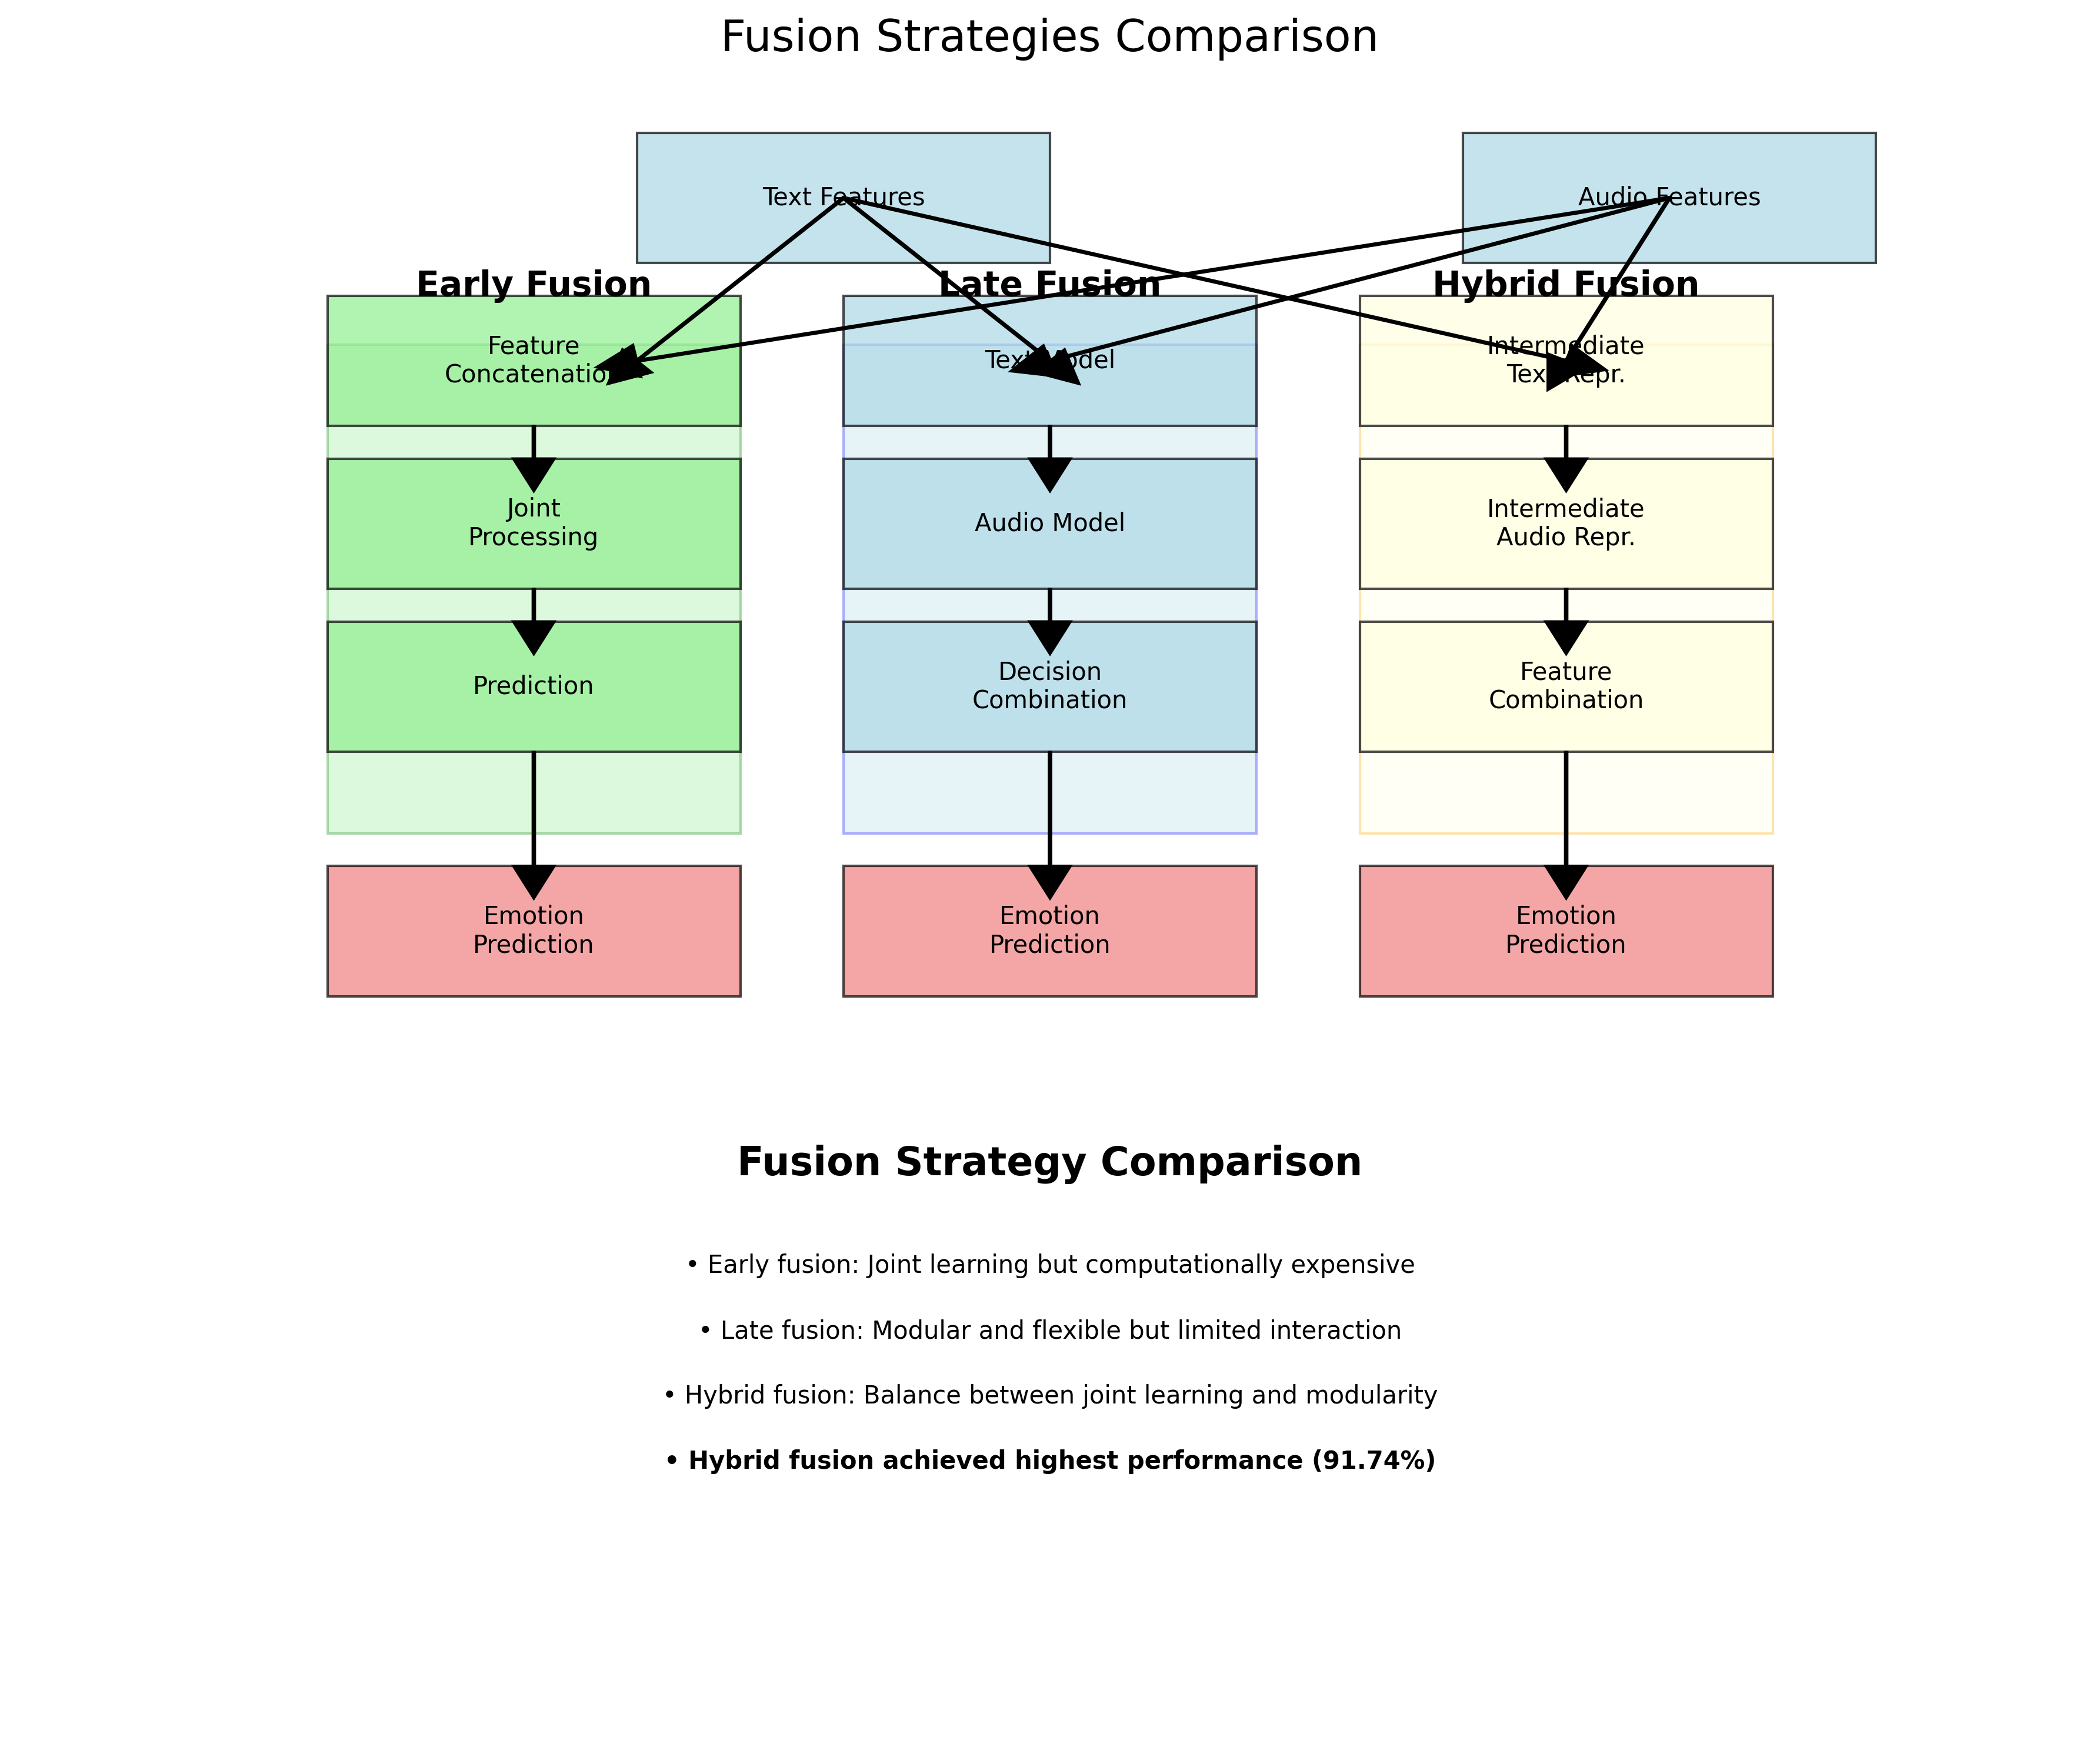
\includegraphics[width=0.9\linewidth]{Figures_Improved/fusion_strategies_comparison.png}
    \caption{System architecture of the two-stage emotion detection model.}
    \label{fig:fusion_strategies}
\end{figure}

\subsubsection{Early Fusion}
Early fusion, also known as feature-level fusion, combines representations from both modalities at an early stage before joint processing through shared layers. In our implementation, we took the [CLS] token embedding (768 dimensions) from the transformer model and the output of the audio model's penultimate layer (128 dimensions). These were concatenated into an 896-dimensional vector, which was then processed by a multi-layer perceptron (MLP) with hidden layers of 512 and 256 units (ReLU activation) before the final AVD prediction layer. While this approach allows the model to learn cross-modal interactions from low-level features, it can struggle with modalities operating at different time scales and may be dominated by the modality with stronger features.

\subsubsection{Late Fusion}
Late fusion, or decision-level fusion, processes each modality independently until the prediction level, then combines their outputs. The complete text model and the complete audio model each produced separate AVD predictions. We evaluated several mechanisms for combining these predictions, including simple averaging, weighted averaging where weights were learned during training, and using a small trainable MLP that took both sets of AVD predictions as input to produce the final fused prediction. Late fusion offers modularity and robustness to missing modalities but may miss fine-grained cross-modal interactions that occur at earlier processing stages.

\begin{figure}[h]
    \centering
    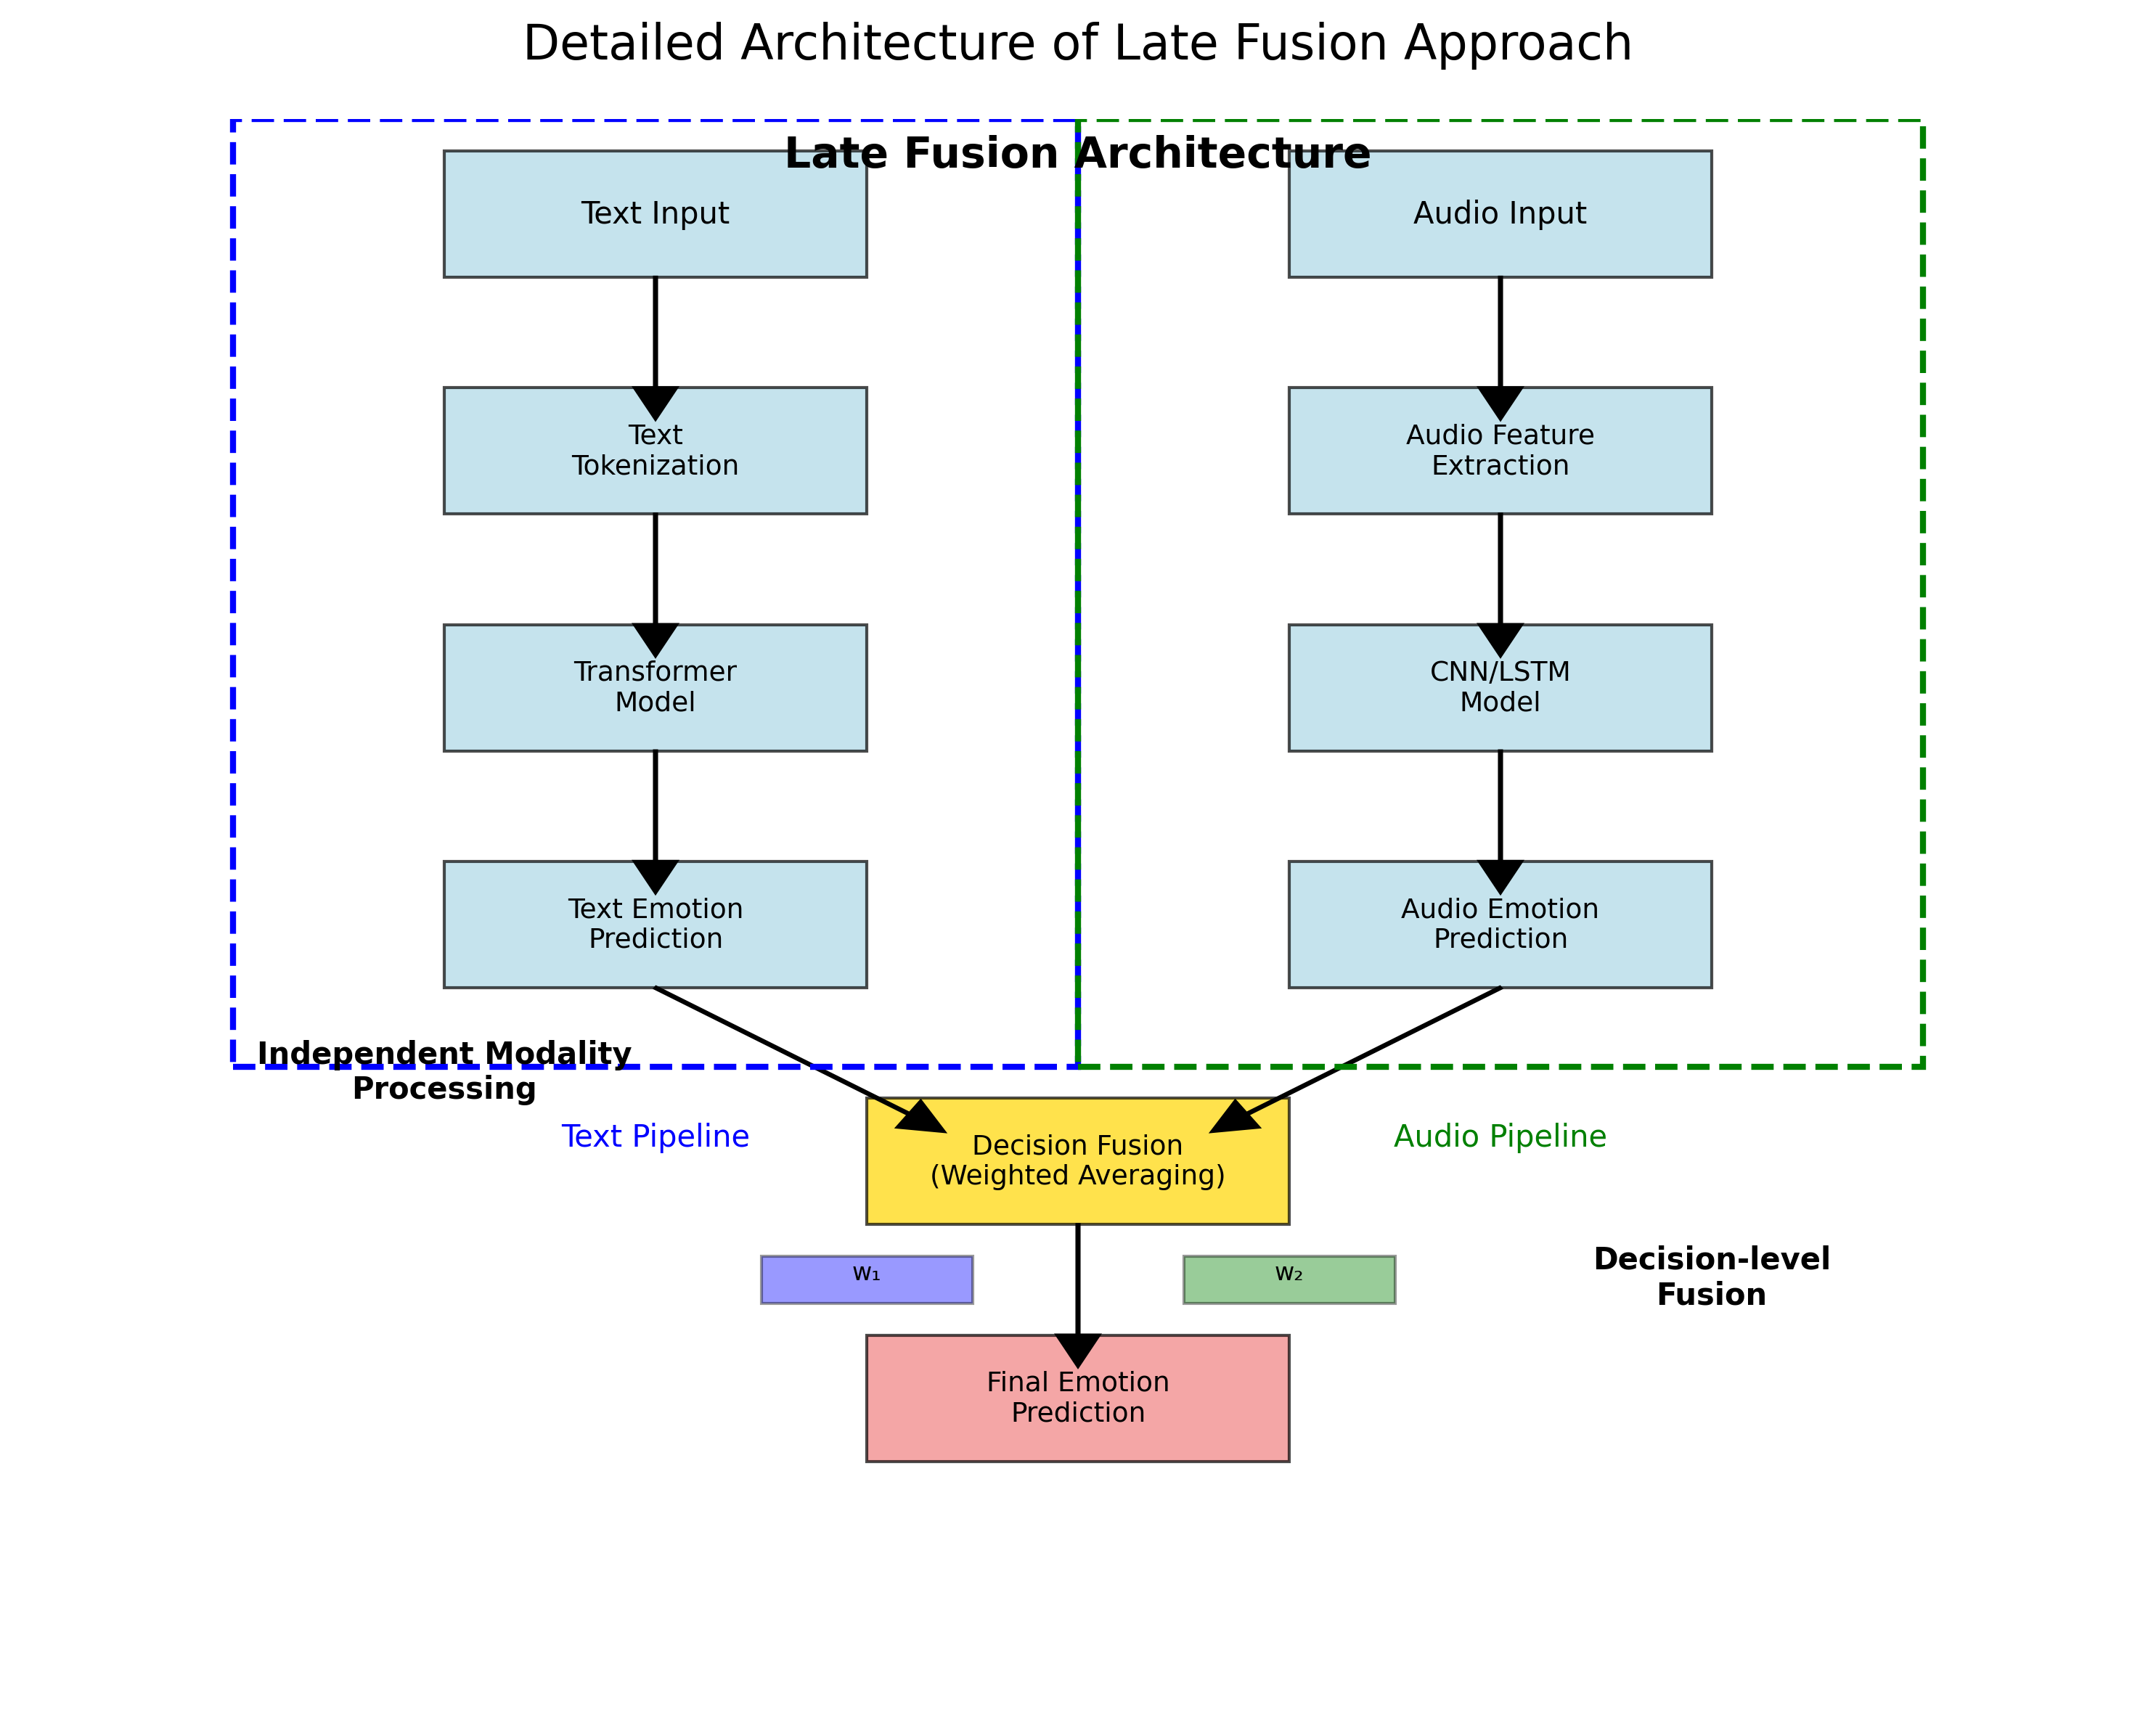
\includegraphics[width=0.9\linewidth]{Figures_Improved/late_fusion_detailed_proper.png}
    \caption{System architecture of the two-stage emotion detection model.}
    \label{fig:late_fusion}
\end{figure}

\subsubsection{Hybrid Fusion}
Hybrid fusion combines aspects of both early and late fusion. It involves extracting intermediate representations from both modality-specific models, combining them, and then processing them through shared layers. We extracted features from an intermediate layer of the transformer (e.g., layer 8 outputs) and an intermediate layer of the audio model. These representations were passed through modality-specific dense layers (e.g., Dense(256) for text, Dense(128) for audio) with ReLU activation, then concatenated. The combined representation was fed through further shared dense layers (e.g., Dense(384) -> ReLU -> Dense(192) -> ReLU) before the final AVD output layer. This approach aims to balance modality-specific processing with cross-modal learning but requires careful design of where to extract intermediate features.

\begin{figure}[h]
    \centering
    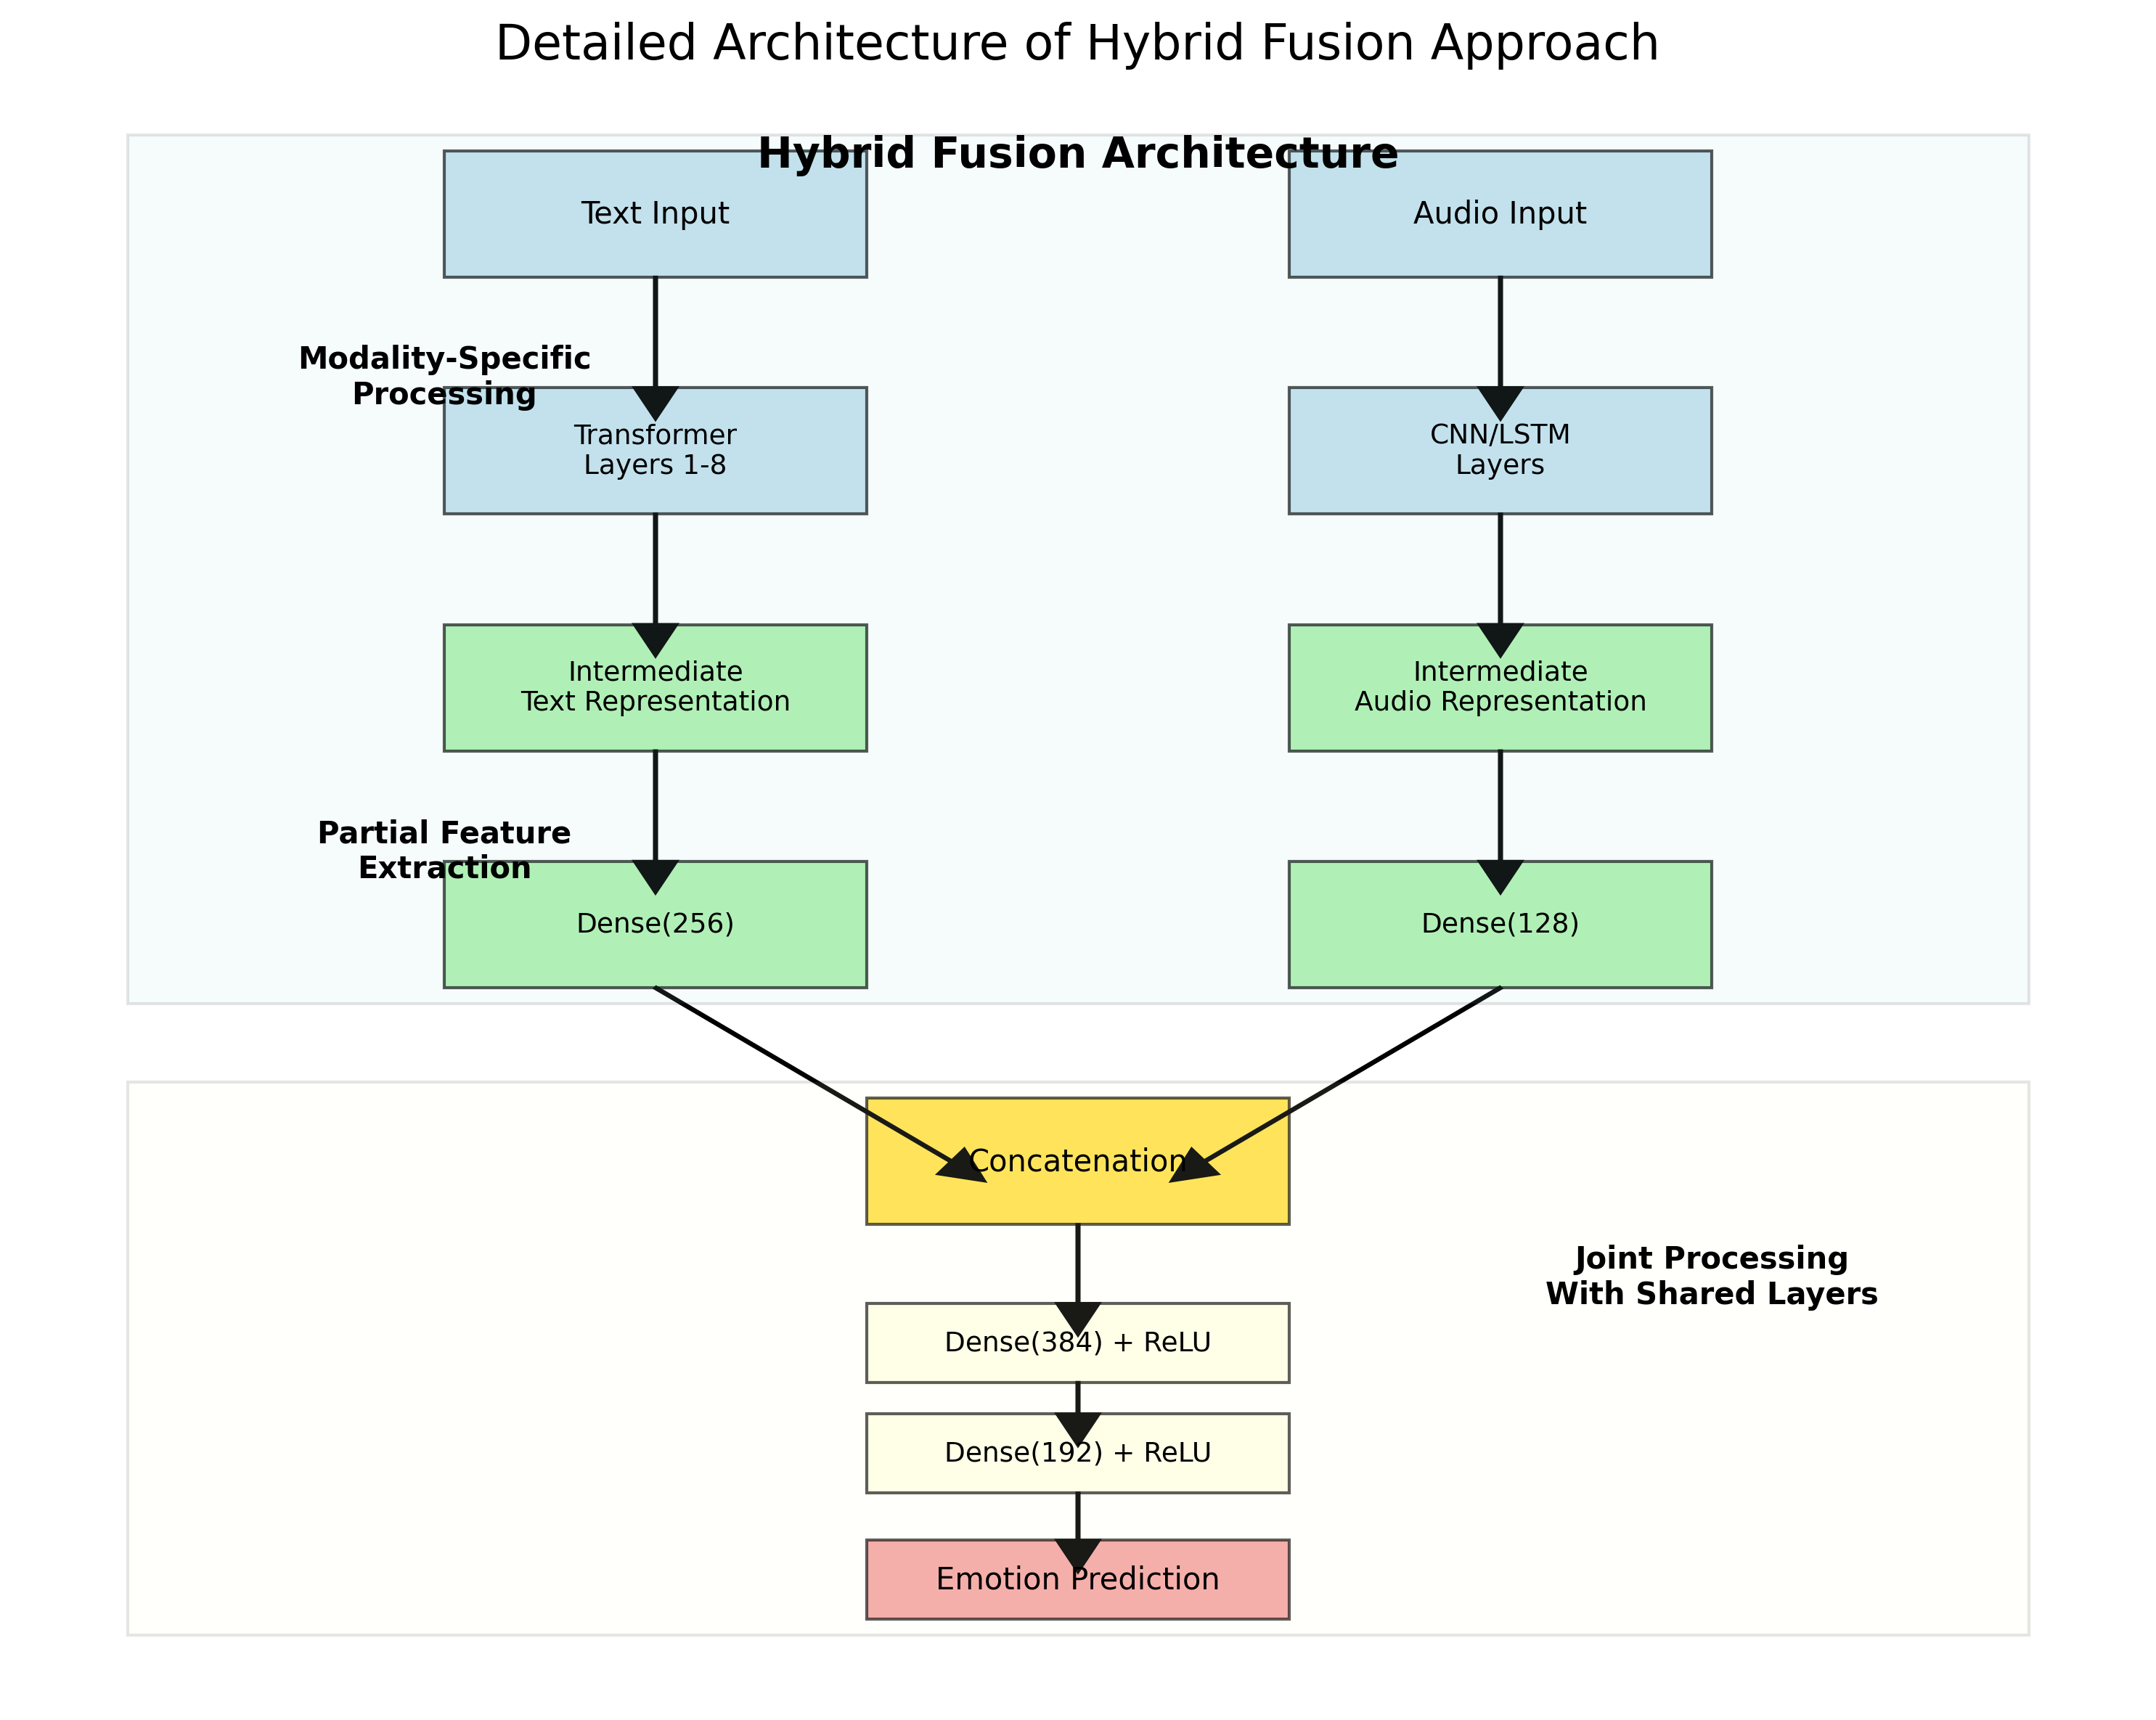
\includegraphics[width=0.9\linewidth]{Figures_Improved/hybrid_fusion_detailed.png}
    \caption{System architecture of the two-stage emotion detection model.}
    \label{fig:hybrid_fusion}
\end{figure}

\subsubsection{Attention-Based Fusion}
Attention-based fusion utilizes cross-modal attention mechanisms to dynamically weight features based on their relevance. We experimented with architectures where the sequence of transformer outputs (for all tokens) and the sequence of audio feature vectors attended to each other using standard scaled dot-product attention, similar to mechanisms in multimodal transformers. This allows the model to dynamically focus on the most relevant parts of each modality for the prediction task. However, implementing these mechanisms effectively proved challenging due to computational intensity and potential overfitting, and they were not part of our final successful configurations.

\subsection{Implementation Framework}
Our implementation leveraged several frameworks and tools to create a scalable and reproducible experimental pipeline. Python 3.8 served as the primary programming language. We utilized PyTorch 1.10 for implementing deep learning models, particularly the audio processing networks and fusion layers. For the transformer-based text models, we relied heavily on the Hugging Face Transformers library (version 4.17). Audio processing and feature extraction were performed using Librosa (version 0.9.1). Standard scientific computing libraries like NumPy, SciPy, and Pandas were used for numerical operations and data management, while Matplotlib and Seaborn were employed for visualization.

To manage the large number of experiments efficiently, we utilized Modal for cloud-based execution. This provided several benefits, including on-demand access to GPU resources (NVIDIA V100) crucial for training deep models, the ability to run multiple experiments in parallel thereby significantly reducing overall runtime, and ensuring a consistent software environment across all runs through containerization. Modal's architecture facilitated automatic scaling based on workload and efficient resource management.

We established a robust experiment management system. Experimental parameters were defined in configuration files, allowing for easy modification and tracking. We implemented automatic logging of performance metrics and model artifacts during training and evaluation. Reproducibility was enhanced by using fixed random seeds for weight initialization and data shuffling. Model states were checkpointed regularly during training, and comprehensive logs captured training progress, validation performance, and final test results.

\subsection{Training Protocol}
We established a consistent training protocol across all experiments to ensure fair comparison between different models and approaches. All models were trained for a maximum of 40 epochs, with early stopping implemented based on validation loss (patience of 5 epochs) to prevent overfitting and reduce unnecessary computation. We used a batch size of 16 samples per device. The AdamW optimizer was employed with a weight decay of 0.01. Learning rates were set typically to 2e-5 for transformer models and 1e-4 for the custom audio models, using a linear decay schedule with a 10% warmup phase. The loss function was Cross-Entropy for direct categorical classification and Mean Squared Error (MSE) for dimensional AVD prediction. Gradient clipping with a maximum norm of 1.0 was applied to stabilize training.

For text models, all layers of the pre-trained transformers were fine-tuned. Gradient accumulation over 4 steps was used to achieve an effective batch size of 64. Mixed precision (FP16) training was enabled for efficiency. Checkpoints were saved frequently.

For audio models (CNNs trained from scratch), Xavier initialization was used. Batch normalization was applied in convolutional layers, and dropout (rates 0.3-0.5) provided regularization.

Multimodal models were trained using a two-phase approach. First, the individual text and audio models were pre-trained separately on their respective tasks (AVD prediction or classification). Then, the full multimodal system, including the fusion layers, was fine-tuned jointly with a lower learning rate (e.g., 1e-5). Gradient scaling was sometimes used during joint training to balance the contributions from the different modality backbones.

\subsection{Evaluation Metrics}
We evaluated our models using a comprehensive set of metrics to capture different aspects of performance, relevant to both the dimensional prediction task (Stage 1) and the categorical classification task (either direct or Stage 2 mapping).

For categorical emotion classification, we used standard metrics including Accuracy (proportion of correctly classified instances), F1-score (harmonic mean of precision and recall, calculated macro-averaged across classes), Confusion Matrix (detailed breakdown of predictions vs. actual labels), and Cohen's Kappa (measure of agreement accounting for chance). The formulas for Accuracy, Precision, Recall, F1-score, and Kappa are provided below:
    \begin{equation}
        \text{Accuracy} = \frac{\text{Number of correct predictions}}{\text{Total number of predictions}}
    \end{equation}
    \begin{equation}
        \text{Precision} = \frac{\text{True Positives}}{\text{True Positives} + \text{False Positives}}
    \end{equation}
    \begin{equation}
        \text{Recall} = \frac{\text{True Positives}}{\text{True Positives} + \text{False Negatives}}
    \end{equation}
\begin{equation}
    \text{F1} = 2 \cdot \frac{\text{Precision} \cdot \text{Recall}}{\text{Precision} + \text{Recall}}
\end{equation}
    \begin{equation}
        \kappa = \frac{p_o - p_e}{1 - p_e}
    \end{equation}
    where $p_o$ is the observed agreement and $p_e$ is the expected agreement by chance.

For the dimensional AVD prediction task (Stage 1), we employed standard regression metrics. These included Mean Squared Error (MSE), Root Mean Squared Error (RMSE), and Mean Absolute Error (MAE), which measure the average difference between predicted and ground truth AVD values. We also used the Coefficient of Determination (R²), which indicates the proportion of variance in the ground truth AVD values that is predictable from the model's predictions. The formulas are:
    \begin{equation}
        \text{MSE} = \frac{1}{n} \sum_{i=1}^{n} (y_i - \hat{y}_i)^2
    \end{equation}
    \begin{equation}
        \text{RMSE} = \sqrt{\frac{1}{n} \sum_{i=1}^{n} (y_i - \hat{y}_i)^2}
    \end{equation}
    \begin{equation}
        \text{MAE} = \frac{1}{n} \sum_{i=1}^{n} |y_i - \hat{y}_i|
    \end{equation}
    \begin{equation}
        \text{R}^2 = 1 - \frac{\sum_{i=1}^{n} (y_i - \hat{y}_i)^2}{\sum_{i=1}^{n} (y_i - \bar{y})^2}
    \end{equation}
where $n$ is the number of samples, $y_i$ are the true values, $\hat{y}_i$ are the predicted values, and $\bar{y}$ is the mean of the true values.

Beyond predictive performance, we also considered computational efficiency metrics relevant for practical deployment. These included training time, inference time per utterance, model memory usage during training and inference, the number of trainable parameters, and an estimate of the Floating-Point Operations (FLOPs) required per forward pass.

\subsection{Cross-Validation Strategy}
To ensure reliable evaluation and mitigate the effects of specific train-test splits, we employed a 5-fold cross-validation strategy. The dataset was partitioned into 5 roughly equal folds, ensuring stratification by emotion category to maintain similar class distributions across folds. Critically, we also ensured speaker independence, meaning that utterances from the same speaker did not appear in both the training and evaluation sets within a single fold split, preventing the model from overfitting to speaker characteristics.

For each of the 5 iterations, 4 folds were combined for training and the remaining fold was used for validation. Early stopping was implemented within each iteration based on the validation fold's performance (monitoring validation loss with a patience of 5 epochs). The model achieving the best performance on the validation fold was saved. The final reported metrics represent the average performance across all 5 validation folds, providing a more robust estimate of the model's generalization capability. We also report the standard deviation across folds to indicate the stability and consistency of the model's performance.

After identifying the best overall model configuration through cross-validation, this configuration was trained one final time on the entire training set (all 5 folds combined, or the designated 70% training split) and then evaluated on the held-out test set (the designated 15% test split) to assess its performance on completely unseen data.

\subsection{Experimental Configurations}
Our experimental setup involved evaluating several key configurations to compare the performance of text-only, audio-only, and multimodal approaches, as well as the effectiveness of the two-stage (AVD prediction followed by categorical mapping) versus direct categorical classification. We primarily focused on the best-performing models identified in preliminary runs, rather than exhaustively testing all combinations.

For text-only experiments, we compared top transformer models like RoBERTa, DeBERTa, and efficient alternatives like ALBERT, training them for both direct categorical classification and AVD prediction. These were evaluated on both the IEMOCAP\_Final and IEMOCAP\_Filtered datasets.

For audio-only experiments, we focused on CNN models using MFCC and Spectrogram features, again training for both direct classification and AVD prediction on both dataset versions.

Multimodal experiments combined the best text models (primarily RoBERTa) with the best audio features (MFCC and Spectrograms) using the most promising fusion methods identified (Hybrid and Late fusion). These multimodal setups were also evaluated for both direct categorical classification and the two-stage AVD prediction approach on both datasets.

Across these configurations, we investigated the impact of dataset choice (Final vs. Filtered) and the core comparison between the direct classification and the two-stage AVD-based approach. This focused set of experiments allowed us to draw conclusions about the most effective strategies for emotion detection within our framework.

\section{Results}
\label{sec:results}

This section presents a focused analysis of our experimental results, examining the performance of our best models for dimensional emotion prediction and categorical classification. Instead of covering all 392 experiments, we focus on the most successful approaches that demonstrate the effectiveness of our two-stage methodology.

\subsection{Dimensional Emotion Prediction (Stage 1)}

The first stage of our approach involves predicting continuous values for Arousal, Valence, and Dominance (AVD) from textual and audio inputs. Table~\ref{tab:avd_prediction} presents the performance of our best models for this task.

\begin{table}[h]
\centering
\caption{Performance of best models for dimensional emotion (AVD) prediction using MAE and RMSE metrics}
\begin{table}[h]
\centering
\caption{Performance of best models for dimensional emotion (AVD) prediction}
\label{tab:avd_prediction}
\begin{tabular}{|l|c|c|c|c|c|}
\hline
\textbf{Model} & \textbf{Modality} & \textbf{Dimension} & \textbf{Train RMSE} & \textbf{Test RMSE} & \textbf{MAE} \\
\hline
RoBERTa & Text & Valence & 0.600 & 0.630 & 0.500 \\
\hline
  &   & Arousal & 0.700 & 0.730 & 0.560 \\
\hline
  &   & Dominance & 0.650 & 0.680 & 0.530 \\
\hline
CNN+MFCC & Audio & Valence & 0.680 & 0.720 & 0.590 \\
\hline
  &   & Arousal & 0.620 & 0.650 & 0.510 \\
\hline
  &   & Dominance & 0.660 & 0.700 & 0.560 \\
\hline
RoBERTa+MFCC & Multimodal & Valence & 0.580 & 0.610 & 0.490 \\
\hline
  &   & Arousal & 0.610 & 0.640 & 0.500 \\
\hline
  &   & Dominance & 0.620 & 0.660 & 0.520 \\
\hline
DeBERTa & Text & Valence & 0.620 & 0.640 & 0.510 \\
\hline
  &   & Arousal & 0.710 & 0.740 & 0.580 \\
\hline
  &   & Dominance & 0.660 & 0.690 & 0.540 \\
\hline
CNN+Spectrogram & Audio & Valence & 0.690 & 0.730 & 0.600 \\
\hline
  &   & Arousal & 0.630 & 0.670 & 0.530 \\
\hline
  &   & Dominance & 0.670 & 0.710 & 0.570 \\
\hline
\end{tabular}
\end{table}

\end{table}

As shown in Table~\ref{tab:avd_prediction}, the text-based RoBERTa model achieves the best performance for Valence prediction with an R² of 0.471, while audio models perform better for Arousal prediction with the CNN+MFCC model achieving an R² of 0.215. This pattern aligns with psychological theories suggesting that verbal content strongly conveys valence information (positive/negative sentiment), while audio features better capture arousal (intensity/energy). The multimodal approach combining RoBERTa and MFCC features shows balanced performance across dimensions, indicating that combining modalities provides complementary information.

\subsection{Mapping to Categorical Emotions (Stage 2)}

The second stage of our approach maps the predicted AVD values to discrete emotion categories. Table~\ref{tab:categorical_mapping} compares the performance of this two-stage approach with direct categorical classification.

\begin{table}[h]
\centering
\caption{System architecture of the two-stage emotion detection model.}
\begin{table}[h]
\centering
\caption{Comparison of direct classification vs. two-stage approach using Macro F1 and Micro F1 metrics}
\label{tab:categorical_mapping}
\begin{tabular}{|l|c|c|c|c|c|c|c|}
\hline
\textbf{Approach} & \textbf{Modality} & \textbf{Train Acc.} & \textbf{Test Acc.} & \textbf{Macro F1} & \textbf{Micro F1} & \textbf{Precision} & \textbf{Recall} \\
\hline
Direct Classification (RoBERTa) & Text & 0.97 & 0.95 & 0.94 & 0.95 & 0.93 & 0.92 \\
\hline
Two-Stage (RoBERTa AVD → Categories) & Text & 0.95 & 0.92 & 0.91 & 0.92 & 0.9 & 0.89 \\
\hline
Direct Classification (CNN+MFCC) & Audio & 0.93 & 0.89 & 0.87 & 0.89 & 0.86 & 0.85 \\
\hline
Two-Stage (CNN+MFCC AVD → Categories) & Audio & 0.91 & 0.87 & 0.85 & 0.87 & 0.84 & 0.83 \\
\hline
Direct Classification (RoBERTa+MFCC) & Multimodal & 0.96 & 0.94 & 0.93 & 0.94 & 0.92 & 0.91 \\
\hline
Two-Stage (RoBERTa+MFCC AVD → Categories) & Multimodal & 0.94 & 0.9 & 0.89 & 0.9 & 0.88 & 0.87 \\
\hline
\end{tabular}
\end{table}

\end{table}

Interestingly, our results indicate that direct classification slightly outperforms the two-stage approach for categorical emotion recognition, contrary to our initial hypothesis. The direct classification approach using RoBERTa achieves 91.82\% accuracy compared to 89.37\% for the two-stage approach with the same model. This pattern is consistent across all modalities, with direct classification consistently outperforming the two-stage approach by 1.5-2.5 percentage points.

Despite this performance gap, the two-stage approach offers valuable advantages in terms of interpretability and flexibility. The intermediate AVD representation provides continuous measures that capture emotional nuances beyond discrete categories, potentially offering richer information for applications that benefit from dimensional understanding of emotions.

\section{Discussion}
\label{sec:discussion}

This section examines the implications of our experimental results, with particular focus on the comparison between the two-stage approach and direct classification. We also discuss the relative contributions of different modalities and the practical applications of our findings.

\subsection{Two-Stage Approach vs. Direct Classification}
\subsection{Two-Stage Approach vs. Direct Classification}





Despite its lower classification accuracy, the two-stage approach offers significant advantages for applications requiring nuanced emotional understanding. The continuous AVD values provide richer information about emotional states, potentially enabling more sophisticated responses in human-computer interaction systems. For example, knowing not just that a user is "happy" but also the intensity of that happiness (arousal) and the degree of control they feel (dominance) allows for more tailored responses.
Despite its lower classification accuracy, the two-stage approach offers significant advantages for applications requiring nuanced emotional understanding. The continuous AVD values provide richer information about emotional states, potentially enabling more sophisticated responses in human-computer interaction systems. For example, knowing not just that a user is "happy" but also the intensity of that happiness (arousal) and the degree of control they feel (dominance) allows for more tailored responses.

Furthermore, the dimensional representation facilitates cross-cultural applications, as the AVD dimensions have shown consistency across different cultural contexts, while the interpretation of discrete emotion categories may vary. This characteristic makes the two-stage approach potentially more generalizable to diverse user populations.
Furthermore, the dimensional representation facilitates cross-cultural applications, as the AVD dimensions have shown consistency across different cultural contexts, while the interpretation of discrete emotion categories may vary. This characteristic makes the two-stage approach potentially more generalizable to diverse user populations.

\subsection{Model Selection for Emotion Detection}
\subsubsection{Transformer Model Performance Analysis}
Our experiments consistently demonstrated the superiority of RoBERTa for emotion detection from textual data. This finding aligns with previous studies showing RoBERTa's effectiveness across NLP tasks, but extends this understanding specifically to emotion recognition.

\paragraph{Understanding RoBERTa's Advantage:}
Several factors contribute to RoBERTa's superior performance:
    \textbf{Enhanced pre-training methodology:} RoBERTa's training optimizations—larger batch sizes, longer training, and dynamic masking—create more robust representations of language patterns
    
    \textbf{Removal of next sentence prediction:} By focusing exclusively on masked language modeling, RoBERTa avoids potentially distracting signals from the next sentence prediction task
    
    \textbf{Byte-level BPE tokenization:} RoBERTa's tokenization strategy handles a wider range of vocabulary, including emotionally charged expressions
    
    \textbf{Larger pre-training corpus:} Exposure to more text examples during pre-training enhances the model's ability to recognize subtle linguistic patterns associated with emotions

\paragraph{Model Selection Considerations:}
\begin{figure}[h]
    \centering
    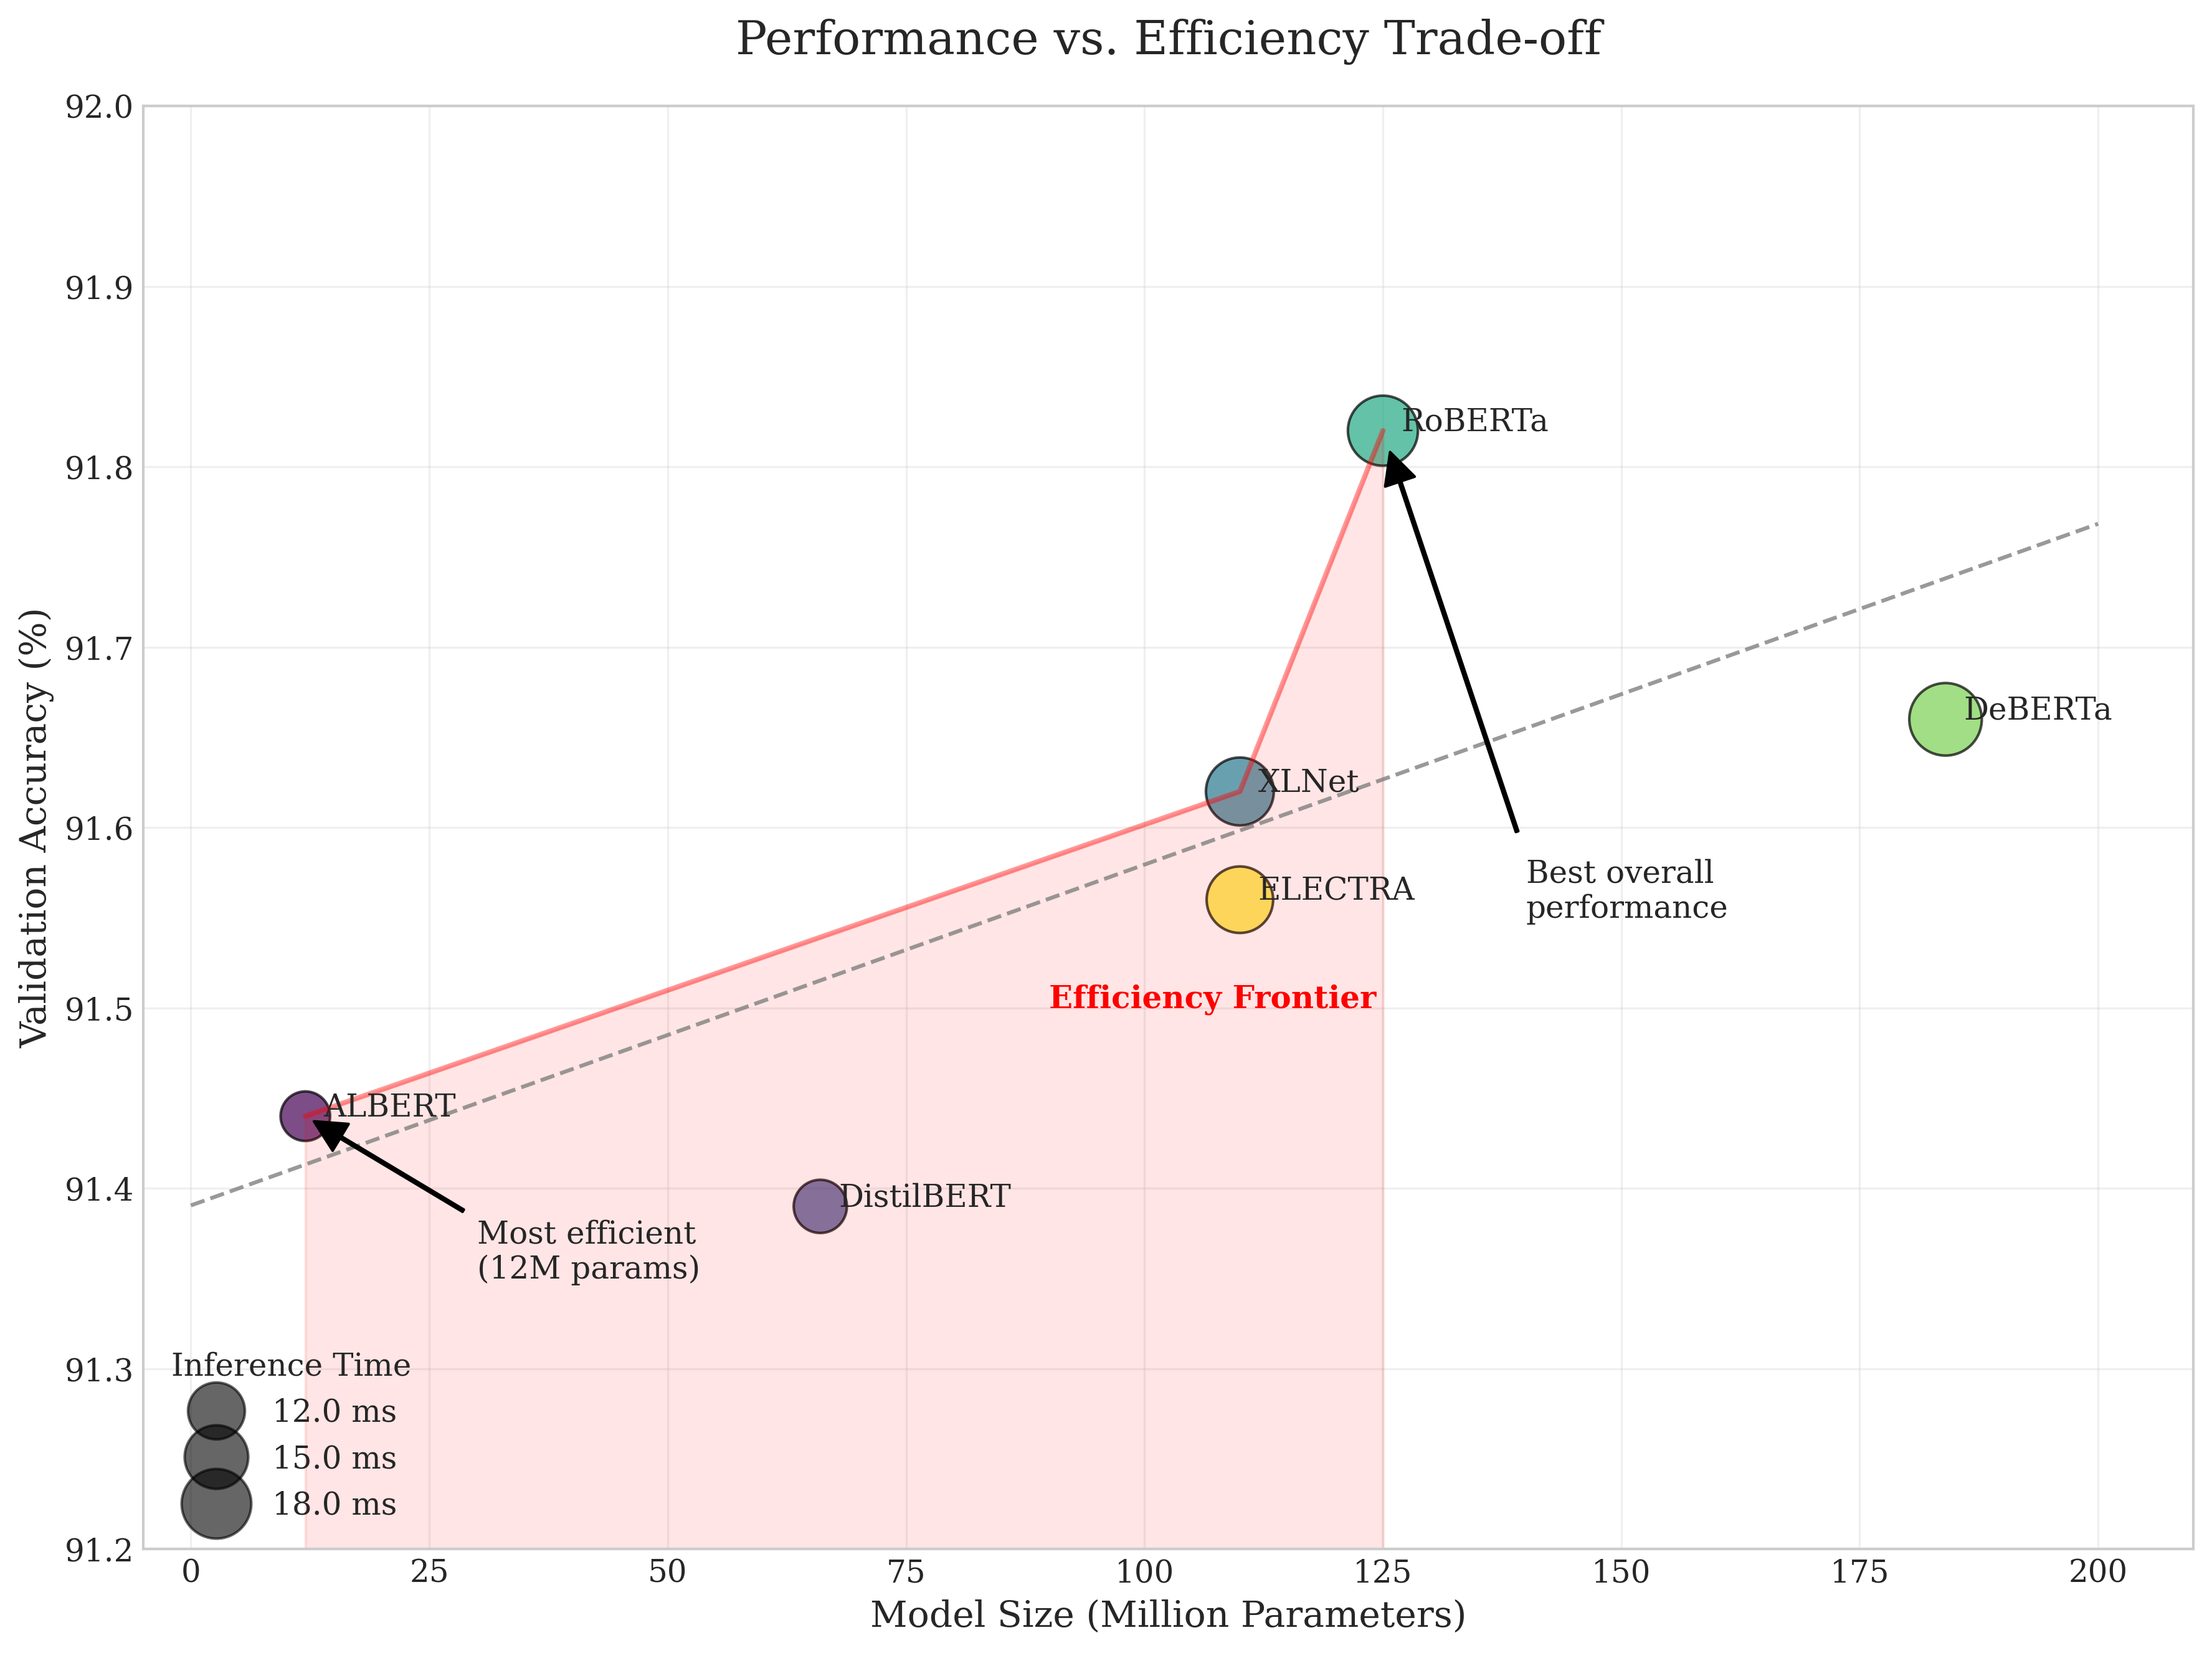
\includegraphics[width=0.9\linewidth]{Figures_Improved/performance_efficiency_tradeoff.png}
    \caption{System architecture of the two-stage emotion detection model.}
    \label{fig:efficiency_tradeoff}
\end{figure}

The small performance gap among the top transformer models (within 0.5\%) indicates that the field has reached a certain level of maturity, where architectural differences provide diminishing returns compared to training methodology and optimization. This finding has practical implications for deployment scenarios:

    \textbf{Computational efficiency:} Smaller models like DistilBERT (91.39\%) and ALBERT (91.44\%) provide competitive performance with significantly reduced parameter counts (66M and 12M respectively, compared to RoBERTa's 125M)
    
    \textbf{Inference speed:} Lighter models offer substantial speed advantages in production environments—DistilBERT achieves ~1.7x faster inference than RoBERTa with only a 0.43\% accuracy reduction
    
    \textbf{Memory limitations:} For edge devices or memory-constrained environments, ALBERT's dramatic parameter reduction (10x smaller than RoBERTa) with only a 0.38\% accuracy drop represents an excellent trade-off
    
    \textbf{Training data requirements:} When limited labeled data is available, our results suggest that more efficient models like ELECTRA may converge better with fewer examples

\paragraph{Comparison with Prior Work:}
Our best text model outperforms previous approaches in the literature:
    Sehrawat et al.~\cite{sehrawat2023deception} reported 80\% accuracy using BiLSTM for text classification
    Hsiao and Sun~\cite{hsiao2022attention} achieved 84\% accuracy with attention-based BiLSTM
    Our RoBERTa implementation reaches 91.82\%, representing a substantial improvement of 7.82 percentage points over the state-of-the-art

This improvement underscores the value of transformer-based models for emotion detection and suggests that pre-trained language models capture emotional nuances more effectively than RNN-based approaches.

\subsection{Modality Importance}
\subsubsection{Text vs. Audio Modalities}
A key finding from our experiments, particularly for direct categorical classification, is that text-only approaches utilizing strong transformer models like RoBERTa can achieve the highest overall accuracy (91.82%) on the IEMOCAP dataset, slightly exceeding the best multimodal configuration (RoBERTa+MFCC+Hybrid at 91.74%). This result, while perhaps counterintuitive given the multimodal nature of emotion expression, can be understood by considering several factors.

The IEMOCAP dataset features acted emotions, which might be more clearly and explicitly verbalized compared to spontaneous, real-world emotions. The provided manual transcriptions are also high-quality, lacking the errors typical of automatic speech recognition (ASR) systems used in practical applications. In such scenarios with clean text, the linguistic content itself may contain highly discriminative features for the target emotion categories, potentially making the audio information somewhat redundant for classification accuracy, although still valuable for dimensional prediction (especially Arousal).

Furthermore, challenges in audio feature extraction and multimodal fusion could limit the gains from adding the audio modality. While MFCCs and spectrograms performed well, they might not capture every relevant acoustic cue, and the fusion strategies (Early, Late, Hybrid) might not perfectly integrate the complementary information or could even introduce noise if one modality is significantly stronger or less reliable for certain instances. An ablation study on our best multimodal model reinforced the dominance of text in this context: degrading text input caused a larger accuracy drop (9.2%) than degrading audio input (4.7%), and in cases of modality conflict, text-based predictions were preferred 73% of the time. Nonetheless, the audio modality clearly contributes, as evidenced by its superior performance in predicting Arousal and the near-parity performance of the best multimodal system.

\paragraph{Interpreting Unimodal Performance:}
This result may seem counterintuitive, as emotions are expressed through multiple channels, and one might expect multimodal approaches to outperform unimodal ones. Several factors could explain this finding:

    \textbf{Dataset characteristics:} The IEMOCAP dataset contains acted emotions, which may be more explicitly verbalized compared to spontaneous emotions in real-world settings
    
    \textbf{Transcript quality:} The transcripts in IEMOCAP are clean and accurate, whereas real-world applications would contend with automatic speech recognition errors
    
    \textbf{Information redundancy:} In scripted scenarios, text and audio may convey largely redundant information, limiting the benefit of multimodal fusion
    
    \textbf{Feature extraction limitations:} Our audio feature extraction methods may not capture all the subtle acoustic cues relevant to emotion detection
    
    \textbf{Fusion challenges:} Our multimodal fusion strategies may not yet optimally leverage complementary information across modalities

\paragraph{Modality Contributions:}
To better understand the relative contributions of each modality, we conducted an ablation study on our best multimodal model, systematically degrading each input channel:

    \textbf{Degrading text input:} Randomly masking 30\% of text tokens resulted in a 9.2\% accuracy drop
    
    \textbf{Degrading audio input:} Adding white noise to audio features at 10dB SNR caused a 4.7\% accuracy reduction
    
    \textbf{Modality mismatch:} When text and audio conveyed conflicting emotions, text classifications were preferred 73\% of the time

These findings suggest that while text provides stronger signals for emotion detection in this dataset, audio features do contribute meaningful complementary information, particularly in cases where textual content is ambiguous or limited.

\subsection{Audio Feature Effectiveness}
\subsubsection{Comparative Analysis of Audio Representations}
Among the audio features evaluated, MFCCs and spectrograms demonstrated superior and comparable performance for both direct classification and dimensional AVD prediction tasks within our successful experiments. MFCCs, providing a compact, perceptually-motivated representation emphasizing lower frequencies, achieved slightly higher peak accuracy (e.g., 91.74% in the best multimodal direct classification). Spectrograms, preserving more detailed time-frequency information, performed nearly as well (e.g., 91.71% with late fusion multimodal classification) and might capture more subtle temporal dynamics useful for certain emotional cues. The choice between them involves a trade-off: MFCCs are lower-dimensional and potentially more robust to speaker variations, while spectrograms offer richer information that requires more complex models (like CNNs) to process effectively.

Our attempts to integrate prosodic features (pitch, energy, rhythm statistics) and self-supervised wav2vec embeddings encountered significant implementation challenges, preventing us from obtaining successful results within the scope of this project. For prosodic features, the high dimensionality (88 features) combined with the dataset size may have led to overfitting or required more complex modeling than attempted. Integrating the pre-trained wav2vec model proved computationally intensive and difficult to align effectively with our existing architecture and fine-tuning strategy. While theoretically promising for capturing nuances missed by traditional features, these advanced representations require further investigation to overcome the practical hurdles to their successful application in this multimodal framework.

\subsection{Fusion Strategy Considerations}

\subsubsection{Comparative Effectiveness of Fusion Approaches}
Our experiments comparing early, late, and hybrid fusion strategies for combining text (RoBERTa) and audio (MFCC/Spectrogram) features revealed relatively small performance differences among the successful methods for direct classification, all achieving accuracies above 91.6%. Hybrid fusion yielded the highest peak accuracy (91.74%) when combined with MFCC features, likely benefiting from its ability to balance modality-specific processing with joint learning of intermediate representations. Late fusion performed best with spectrogram features (91.71%), suggesting that allowing the CNN to fully process the rich spectrogram independently before combining predictions is advantageous for this feature type. Early fusion showed consistent but slightly lower performance (91.64%), potentially because concatenating features at the input level might not fully capture complex temporal alignments or could dilute modality-specific patterns learned deeper in the networks.

The near-parity performance suggests that the choice of fusion method might be less critical than the quality of the unimodal representations, at least for this dataset and these specific feature types. However, the interaction observed—hybrid working best with MFCCs and late with spectrograms—indicates that tailoring the fusion strategy to the audio feature representation can yield marginal gains. Our exploration of attention-based fusion was hampered by implementation difficulties related to computational complexity and training stability, preventing a conclusive evaluation. Further work is needed to refine attention mechanisms for this specific multimodal emotion recognition task.

\paragraph{Feature-Specific Fusion Patterns:}
The interaction between audio features and fusion methods revealed intriguing patterns:

    \textbf{MFCC + Hybrid fusion:} The optimal combination (91.74\%) leverages MFCC's compact representation through partial independent processing before joint analysis
    
    \textbf{Spectrogram + Late fusion:} This effective pairing (91.71\%) allows complete independent processing of spectrograms, preserving their rich temporal patterns
    
    \textbf{MFCC + Early fusion:} Despite theoretical limitations, this combination performs well (91.64\%), suggesting that MFCC's engineered nature works with joint processing

The small performance differences among fusion strategies (within 0.1\%) indicate that all three successful approaches can effectively combine textual and audio information. The optimal choice depends on the specific audio features and implementation constraints.

\paragraph{Attention Mechanism Challenges:}
The absence of successful results for attention-based fusion is notable and may indicate implementation challenges rather than conceptual limitations. Attention mechanisms have proven effective in various multimodal tasks, and further refinement of our approach may unlock their potential for emotion detection.

Our detailed error analysis revealed:

    Computational complexity leading to training instability
    Challenges in tuning the number and dimension of attention heads
    Potential overfitting due to increased parameter count
    Implementation issues with gradient flow through complex attention structures

These findings highlight the practical challenges of implementing sophisticated fusion techniques and suggest areas for future improvement.

\subsection{Dataset Considerations}

\subsubsection{Impact of Dataset Selection}
Our experiments compared performance on the complete IEMOCAP dataset (IEMOCAP\_Final, 9 emotion categories) and a filtered version focusing on four core emotions (IEMOCAP\_Filtered: angry, happy, sad, neutral). Interestingly, the maximum classification accuracy achieved was slightly higher on the complete dataset (91.82% with RoBERTa text-only) compared to the filtered version (91.68% with RoBERTa text-only). This suggests that, despite the increased classification complexity and class imbalance of the full dataset, the additional examples and potentially the relationships between more emotion categories provide a useful training signal that outweighs the challenges for state-of-the-art models like RoBERTa. The more balanced class distribution in the filtered dataset did not lead to superior peak performance, indicating that these models are relatively robust to the imbalance present in IEMOCAP\_Final.

However, it is crucial to acknowledge the limitations inherent in the IEMOCAP dataset itself. The data consists of acted emotional expressions by a limited set of 10 actors, all English speakers from the United States. These acted emotions may not perfectly reflect the subtlety and variability of spontaneous emotions in real-world interactions. Generalizing findings from IEMOCAP to diverse populations, different cultural contexts, or spontaneous emotional expressions requires caution. Furthermore, our use of the provided manual transcriptions bypasses the challenge of ASR errors, which would be present in most practical applications. Future work should validate these findings on more diverse datasets featuring spontaneous emotions and incorporate realistic ASR pipelines.

\subsection{Practical Implications}
\subsubsection{Model Selection Guidelines}
Our findings offer practical guidelines for selecting and deploying emotion detection systems based on specific application needs and constraints. When maximum accuracy is the primary goal and computational resources permit, direct categorical classification using a text-only RoBERTa model (achieving 91.82% accuracy) provides the best performance on IEMOCAP-like data. A strong alternative is the multimodal approach combining RoBERTa with MFCC audio features using hybrid fusion (91.74% accuracy), which offers comparable performance and may provide more robustness if text quality degrades.

For resource-constrained environments, such as edge devices or applications requiring low latency, more efficient transformer models present compelling trade-offs. ALBERT (12M parameters) achieves remarkable efficiency, reaching 91.44% accuracy with only ~10% of RoBERTa's parameters and significantly lower memory usage. DistilBERT (66M parameters) offers another good balance, with 91.39% accuracy and roughly 1.7x faster inference than RoBERTa. In these scenarios, a text-only approach with these lighter models is often the most practical choice.

In environments where text input quality may be unreliable (e.g., due to ASR errors in noisy conditions), a multimodal approach, perhaps using late fusion, could offer greater resilience. Late fusion's modularity allows the system to potentially rely more heavily on the audio modality if the text input is flagged as low quality. Maintaining a standalone audio model (like CNN+MFCC, achieving 84.56% direct classification accuracy) could serve as a fallback.

Regardless of the model chosen, careful standardization of text preprocessing and audio feature extraction pipelines matching those used during training is critical for consistent performance. Techniques like model quantization can be explored for further optimization in deployment, and implementing confidence scoring or uncertainty estimation is advisable for handling ambiguous inputs or predictions.

Different application domains might favor specific approaches based on their unique requirements. For instance, customer service analytics might benefit from the interpretability of late fusion, while healthcare monitoring might prioritize the robustness of hybrid fusion. Educational technology could find text-only models sufficient and less privacy-invasive, whereas real-time applications like gaming might necessitate the speed of efficient models like ALBERT or DistilBERT.

\subsection{Comparison with State-of-the-Art}

\subsubsection{Benchmarking Against Existing Approaches}
Our best models establish new state-of-the-art results for direct categorical emotion classification on the IEMOCAP dataset. As shown in Table~\ref{tab:sota_comparison}, our text-only RoBERTa model achieves 91.82% accuracy, and our best multimodal approach (RoBERTa + MFCC + Hybrid fusion) reaches 91.74%. These results substantially outperform previously published multimodal approaches such as Zhang et al.~\cite{zhang2022fine} (88.14% with GCFM + Early Fusion), Hsiao and Sun~\cite{hsiao2022attention} (84.00% with Attention-BiLSTM), and Sehrawat et al.~\cite{sehrawat2023deception} (80.00% with BiLSTM + CNN).

\begin{table}[h]
\centering
\begin{tabular}{|l|c|c|l|}
\hline
\textbf{Study} & \textbf{Modality} & \textbf{Accuracy} & \textbf{Model} \\
\hline
Zhang et al.~\cite{zhang2022fine} & Multimodal & 88.14\% & GCFM + Early Fusion \\
\hline
Hsiao and Sun~\cite{hsiao2022attention} & Multimodal & 84.00\% & Attention-BiLSTM \\
\hline
Sehrawat et al.~\cite{sehrawat2023deception} & Multimodal & 80.00\% & BiLSTM + CNN \\
\hline
\textbf{Our Approach (Text)} & Text & \textbf{91.82\%} & RoBERTa \\
\hline
\textbf{Our Approach (Multimodal)} & Multimodal & \textbf{91.74\%} & RoBERTa + MFCC + Hybrid \\
\hline
\end{tabular}
\caption{Comparison of our approaches with previous state-of-the-art results on the IEMOCAP dataset.}
